
\chapter{SYSTEM ANAYLYSIS}
\section{Market Survey}
To comprehend the scope and orientation of the system, it’s essential to conduct a market survey of similar systems. Pet adoption systems, each with its unique features and benefits, come in various forms. In Vietnam, however, most organizations in this field operate through social network pages like Facebook and Instagram, rather than standalone software systems. Notably, the only pet adoption system that stands out from the rest is Hanoi Pet Adoption, which warrants further analysis and evaluation.

\subsection{Overview}
The Hanoi Pet Adoption (HPA) system, a web application based in Hanoi, Vietnam, serves as a platform for individuals to find and adopt rescued animals. The primary objective of this system is to aid the HPA group in rescuing and caring for animals, and subsequently finding them loving and responsible homes.

HPA has the following main features:
\begin{itemize}
  \item \textit{Pet profiles:} The system showcases profiles of animals ready for adoption. These profiles include details such as photos, names, genders, ages, colors, and sterilization statuses.
  \item \textit{User Preferences:} Users can filter animals based on their preferences, including gender, age, color, and sterilization status.
  \item \textit{Volunteer Contact Information:} The system provides the contact information of volunteers responsible for each animal, enabling users to inquire further about their animal of interest.
  \item \textit{Adoption Process Guidance:} The system guides users through the adoption process, which includes an interview, a contract, and a fee.
\end{itemize}

\subsection{Evaluation}
HPA provides a comprehensive and effective pet adoption support process. However, its limitation lies in its exclusivity - only system administrators of the organization are permitted to post pet profiles onto the system.

The absence of a messaging system in the current platform can create challenges in the pet adoption process. This lack of direct communication makes it difficult for system administrators and users to contact each other, particularly when issues arise. A messaging system would facilitate smoother interactions and problem resolution, enhancing the overall user experience.

Currently, the system requires manual input for posting, filtering, and searching functions. This can pose challenges for individual users, potentially reducing the efficiency of posting and searching, and negatively impacting the user experience.

Lastly, a significant feature that is absent in the system is a notification system. Such a system would alert users when pets that meet their criteria are posted, ensuring that users are promptly informed about potential matches. This feature could greatly enhance the user experience and effectiveness of the pet adoption process.

\subsection{Potential Improvements}
After a thorough review of the strengths and weaknesses of existing systems, we have identified several potential enhancements that could significantly improve the user experience and functionality of the system.

Firstly, we propose to \textbf{expand the HPA system}. Currently, the pets are only posted by system administrators. However, SGT aims to allow individuals wishing to surrender their pets to proactively post about their pets for adoption. This expansion would not only increase the number of pets available for adoption but also provide a platform for pet owners and organizations to share valuable information and updates about their pets.

Secondly, we suggest the implementation of \textbf{interactive pet profiles}. This feature would allow users to visit and interact with pet profiles and posts. This interaction could include liking, commenting, or sharing a pet’s profile.

Next, we recommend \textbf{applying Artificial Intelligence (AI) technology to enhance the posting and searching} functionality of the system. With this feature, users could simply upload a pet image, and the AI would automatically populate most of the input fields, such as breed, and color. This would not only simplify the process of posting a pet profile but also increase the accuracy and consistency of the pet information in the system.

In addition, we propose the implementation of a \textbf{notification system}. This system would alert users when a pet that matches their preferences becomes available on the system. User criteria for filtering pet profiles(such as breed, age, or size) will be referenced, and then users can receive notifications when a matching pet is posted. This would ensure that users don’t miss out on potential matches and can act quickly to adopt their desired pet.

Lastly, we suggest establishing a \textbf{messaging system} that facilitates communication among pet adopters, pet owners, and system administrators. This system would allow users to ask questions, clarify information, or arrange meetings, enhancing the overall user experience and streamlining the adoption process. By providing a platform for direct communication, we can foster a sense of community among users and promote open and transparent discussions about pet adoption.

In conclusion, these enhancements aim to make the system more user-friendly, efficient, and effective in connecting pets with potential adopters. We believe that by implementing these changes, we can take a significant step toward our goal of finding a loving and suitable home for every pet.

\section{Stakeholders}
Stakeholders for a project focused on creating a pet adoption platform in Vietnam would include a diverse range of individuals, organizations, and groups with an interest in or influence over the project. Here are some key stakeholders:
\begin{itemize}
  \item \textit{Administrator:} The administrator is responsible for managing and overseeing the platform's operations. They have control over user accounts, content moderation, and the overall functionality of the website.
  \item \textit{Pet Adopter:} Pet adopters are individuals looking to provide a loving home to pets available for adoption. They may already own pets or be first-time pet owners. Pet adopters interact with pet owners and adoption agencies through messaging and inquiries about available pets. They can also share their adoption stories and experiences with the platform's community.
  \item \textit{Pet Owner:} Pet owners are individuals who currently own and care for pets, including dogs, cats, or other animals. Or those, for various reasons, have decided to give their pets to new homes. Reasons may include relocation, financial constraints, allergies, or changes in life circumstances.
  \item \textit{Guest:} Guests are individuals who visit the platform without creating an account or logging in. They have limited access to platform features and content. Guests can browse public content, view pet listings, read provided blogs, and explore the platform's resources. They can also choose to create an account to access more features.
  \item \textit{Pet Adoption Agencies and Shelters:} Organizations involved in pet adoption, rescue, and rehoming would benefit from the platform as it could help them find suitable homes for abandoned or rescued animals. They might also contribute content and listings.
  \item \textit{Pet-Related Businesses:} Pet stores, pet food suppliers, grooming salons, veterinary clinics, and other businesses in the pet industry have a stake in the project. They could use the platform to advertise their products and services to a targeted audience.
  \item \textit{Veterinarians:} Veterinarians play a crucial role in pet healthcare. They might use the platform to provide information, answer questions, and offer telehealth services. Their expertise can be valuable to pet owners.
  \item \textit{Investors and Funders:} Individuals or organizations providing funding or investment for the development and scaling of the platform are stakeholders with a financial interest.
\end{itemize}

Understanding and engaging with these stakeholders will be important for the success and sustainability of the project. Each stakeholder group may have different needs, interests, and concerns that should be addressed during the project's planning and execution.

\section{Requirements eliciation}
\subsection{Functional Requirements}

\begin{longtblr}[
    caption = {Functional Requirements},
    label = {tblr:func_req},
  ]{
    vline{1-3} = {-}{},
    hline{-} = {1-2}{},
    colspec={X[2,l] X[5, l]},
  }
  \textbf{Group}                                & \textbf{Requirements}                                                                                                                                                                                                                                                                                                                                                                                                                                                                                                                                                                      &  &  \\
  \textbf{Authentication and authorization}     & {
    -~~~~~~~
    Users can create new accounts by providing personal information.
    \\-~~~~~~~
    Users can log into the system using Google accounts.
    \\-~~~~~~~
    Users can log into the system by
    providing a registered email and password.
    \\-~~~~~~~
    Users can send applications to the system to update their accounts to
    Organization accounts.
    \\-~~~~~~~
    Admins can verify Organizations’ registration and upgrade users’
    accounts.
    \\-~~~~~~~
    Users can reset or recover their account passwords.
    }                                                          &  &  \\
  \textbf{Pet profile management}               & {
    -~~~~~~~
    Users can create pet profiles by giving details such as name, species,
    breed, age, color, health status, sterilization status, pictures, and videos
    of pets.
    \\-~~~~~~~
    Users can provide information about breed, species, and color by
    uploading pets’ pictures.
    \\-~~~~~~~
    Pet photos and text inputs must be sensitive-validated before
    uploading.
    \\-~~~~~~~
    Users can edit their pet profiles.
    \\-~~~~~~~
    Users can publish, hide, or remove their pet profiles.
    \\-~~~~~~~
    Admins can remove or hide any pet profiles of the system.
    } &  &  \\
  \textbf{Pet profile filter and view}          & {
    -~~~~~~~
    Users can search for pets by providing filtering options such as name,
    species, breed, age, color, health status, and sterilization status.
    \\-~~~~~~~
    Users can search for pets by providing pets’ pictures.
    \\-~~~~~~~
    Users can view pet profiles with detailed information such as name,
    species, breed, age, color, health status, sterilization status, pictures,
    and videos of pets
    }                                                                                                                                                                &  &  \\
  \textbf{Pet adoption}                         & {
    -~~~~~~~
    Users can submit applications to adopt pets on the system.
    \\-~~~~~~~
    Users can view, decline, or accept adoption applications sent to their
    pets.
    }                                                                                                                                                                                                                                                                                                                                                                                                                &  &  \\
  \textbf{User interaction and engagement}      & {-~~~~~~~
  Pet
  Adopters can send messages to Pet Owners, Organizations, and Admins.
  \\-~~~~~~~PetAdopters have to update their pets’ status every seven days[1]~ from the date they received the petsby uploading posts in the adopt status section of the pet profile.\\-~~~~~~~
  Pet
  Adopters can set their posts public for all users or just Admins, and Pet
  Owners.
  \\-~~~~~~~
  Admins
  and Pet Owners can view and interact with posts from Pet Adopters.
  \\-~ ~ ~ ~ All users of the system can view and interact
  with posts from Pet Adopters if the posts are public.~ ~ ~~}        &  &  \\
  \textbf{Blog management}                      & {
    -~~~~~~~
    Admins and Organizations can create and publish blogs.
    \\-~~~~~~~
    Organizations can apply advertisements on their blogs.
    \\-~~~~~~~
    Organizations can edit or remove their blogs.
    \\-~~~~~~~
    Admins can hide or remove any blogs of the system.
    }                                                                                                                                                                                                                                                                                                             &  &  \\
  \textbf{Advertisement and payment}            & {
    -~~~~~~~
    Organizations can choose advertisement duration with different prices.
    \\-~~~~~~~
    Organizations can pay advertisement fees through an online banking
    service.
    \\-~~~~~~~
    Admins can receive advertisement fees through an online banking
    service.
    \\-~~~~~~~
    System provides admins and organizations information like payment
    status and invoices.
    }                                                                                                                                                                                                   &  &  \\
  \textbf{Notifications}                        & {
    -~~~~~~~
    Users can receive notifications on new pet adoption applications.
    \\-~~~~~~~
    Users can receive notifications on new pets’ status posts uploaded.
    \\-~~~~~~~
    Users can receive notifications on new pet profiles matching their
    criteria.
    }                                                                                                                                                                                                                                                                                                                      &  &  \\
  \textbf{System statistics for administrators} & -~~~~~~~
    Admins can get statistics about systems usages, such as the number of
    pet profiles, adopted pets; number of users and Organizations; number of
    blogs, and the total amount of advertisement fee.                                                                                                                                                                                                                                                                                                                                                                            &  &  
\end{longtblr}


\subsection{Non-Functional Requirements}
\section{Use-case analysis}
\subsection{The whole system}
\subsection{Login}
\subsection{Register}
\subsection{Update to organization account}
\subsection{Mange pet profile}
\subsection{Access pet profile}
\subsection{Adopt pets}
\subsection{Update pet status}
\subsection{Interact with pet posts}
\subsection{Make payement}
\subsection{Manage blogs}

\section{Workflow analysis}
\subsection{Activity Diagrams}

\textbf{Self Registration}

The use case starts when a user accesses the register page (or clicks the register button on the login form), and then a register form will be displayed. The user provided some information (including email, password, and name). Then,  the provided information is verified. If it is valid, a confirmation email will be sent to the user. After accessing the link in the email, a new account is created and the user can log into the system.

\begin{figure}[H]
  \centering
  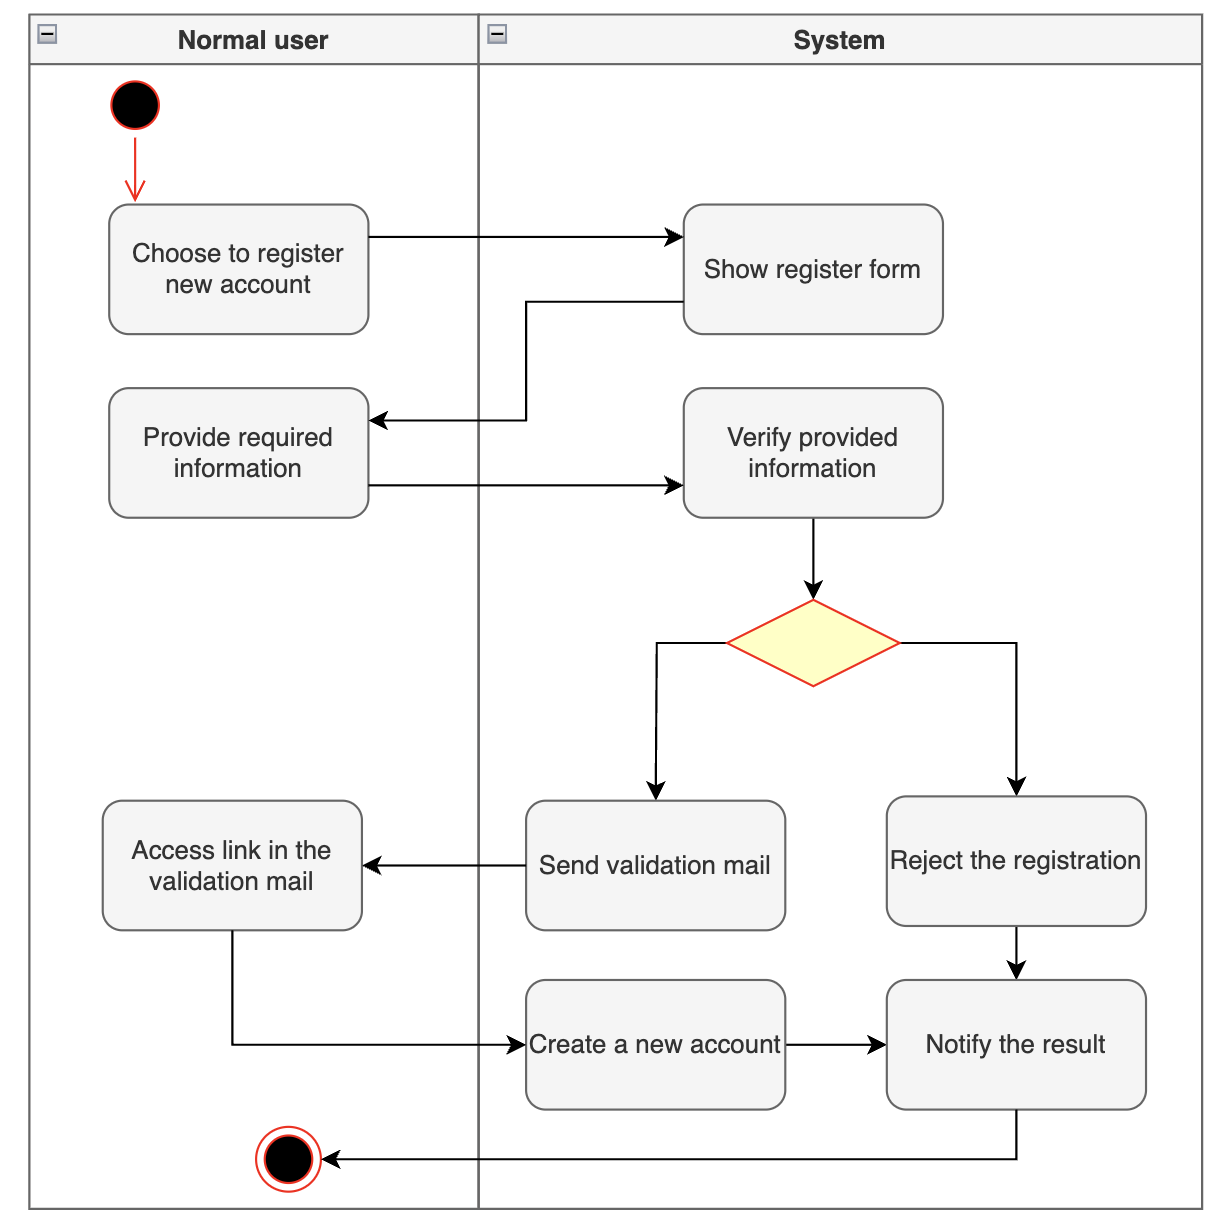
\includegraphics[width=0.7\textwidth]{Figures/self_register.png}
  \caption{Self Registration activity diagram}
  \label{fig:self-registration}
\end{figure}


\textbf{Login}

The use case starts when an unauthorized user tries to access internal features or goes to the login page. The user at the login can provide an email and password and send them to the system. If the credential information is valid, the user will be granted access permission and navigated to an internal page. Otherwise, an error alert will be displayed.

\begin{figure}[H]
  \centering
  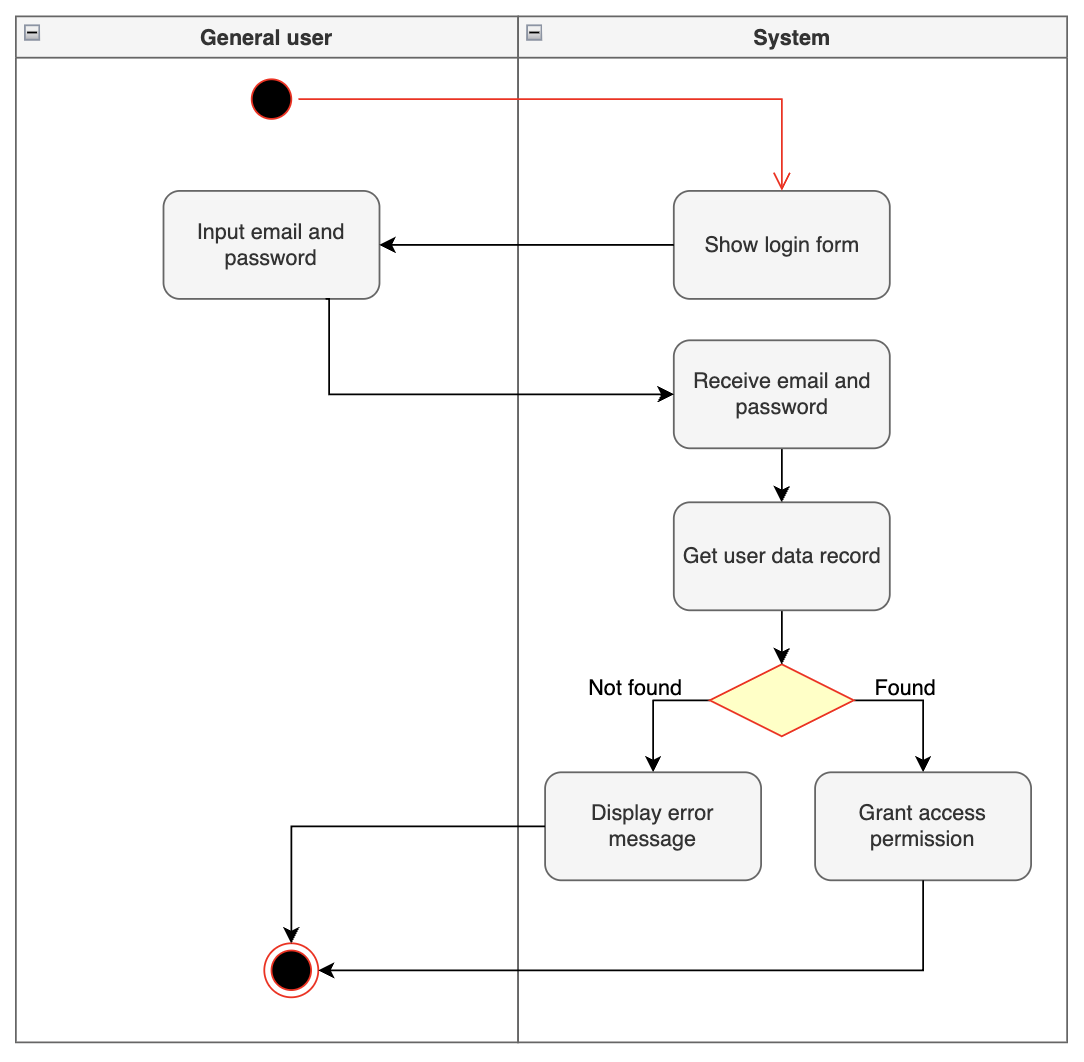
\includegraphics[width=0.7\textwidth]{Figures/login.png}
  \caption{Login activity diagram}
  \label{fig:login}
\end{figure}

\textbf{Login with a Google account}

The use case starts when a user chooses the option of logging in with a Google account, then a Google login form will be displayed. Users provide Google authentication information. Google Auth service verifies the authentication information and generates an access token. Finally, the system validates the access token and grants access permission to the user.

\begin{figure}[H]
  \centering
  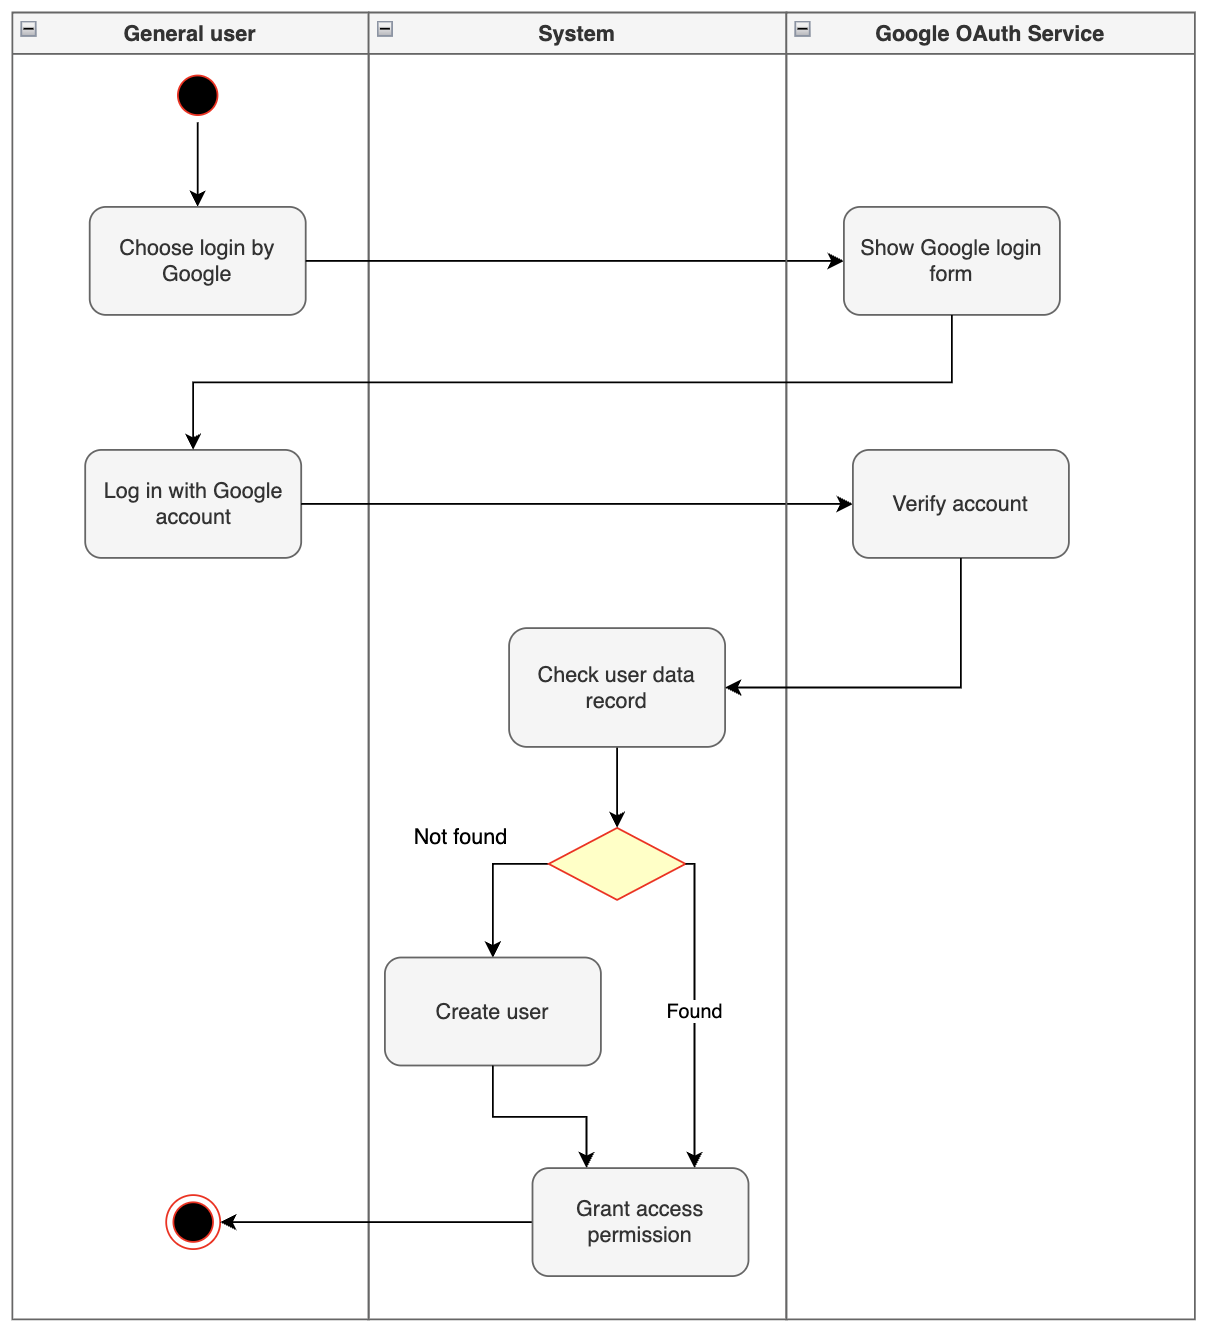
\includegraphics[width=0.7\textwidth]{Figures/login_gg.png}
  \caption{Login with a Google account activity diagram}
  \label{fig:login-google}
\end{figure}

\textbf{Update to Organization account}

The use case starts when an individual user chooses to update to organization accounts, then a form will be displayed. Then, users provide some information for verification and submit them. After the update-account application is verified by admins, the system updates the account and notifies the user of the results.

\begin{figure}[H]
  \centering
  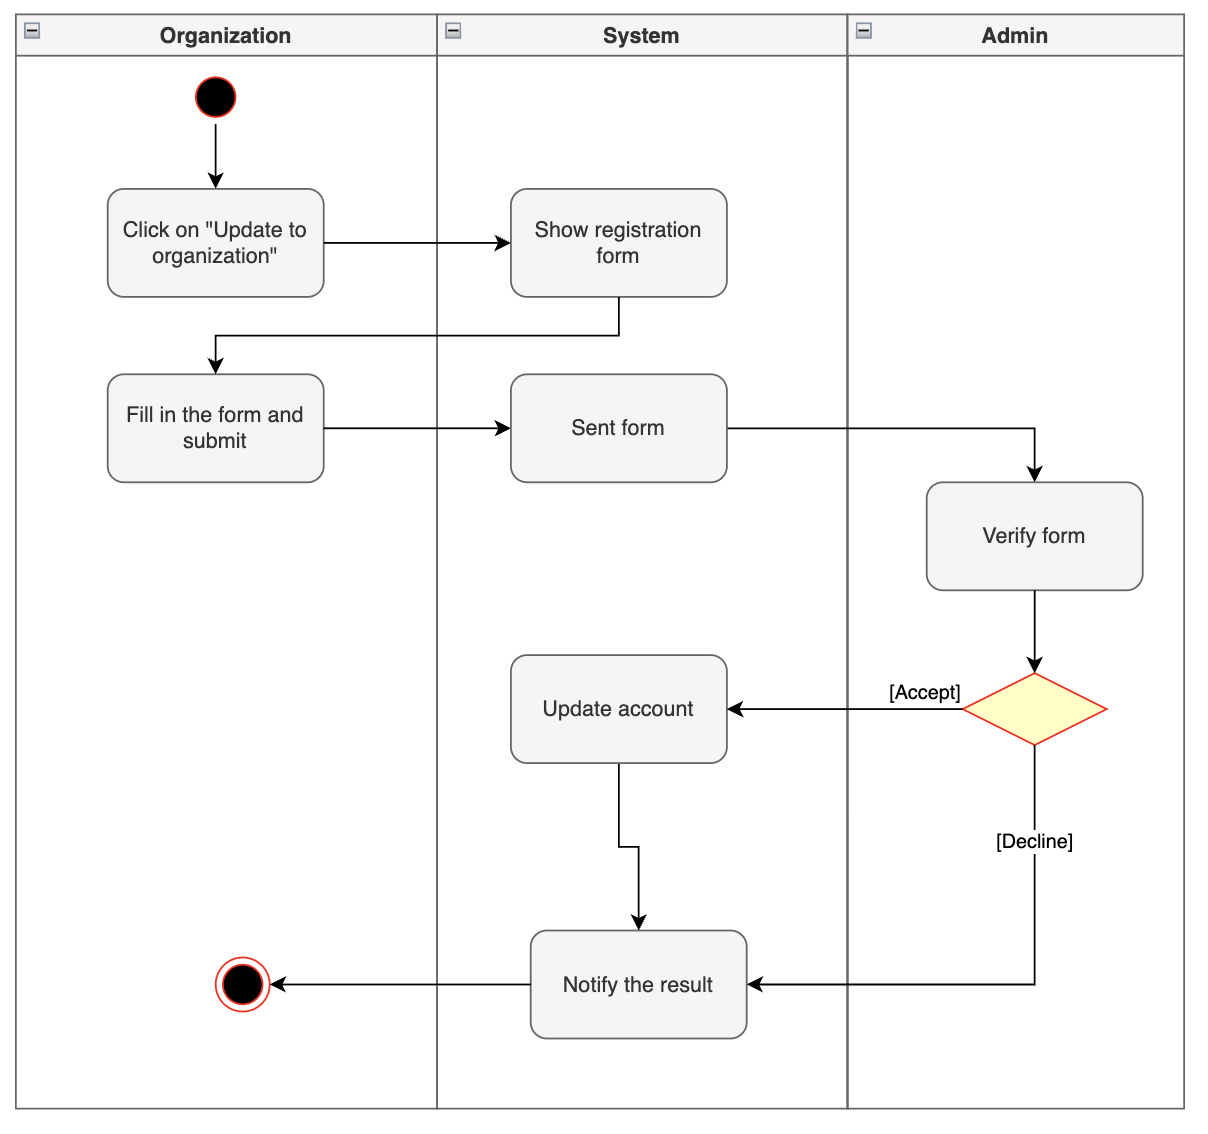
\includegraphics[width=0.7\textwidth]{Figures/update_org.png}
  \caption{Update to Organization account activity diagram}
  \label{fig:update-org}
\end{figure}

\textbf{Manage pet profile}

The use case starts when a user accesses the pet profile management page. The user chooses to edit or create a new profile and a form will be displayed. Note that the form would be filled if the user chose to edit an available profile. In that case, the user can modify the fields or rather delete the profile. Otherwise, the user can input the pet information and submit it. The user can also fill in pet breeds and colors by providing images. Finally, the content of the form will be verified, and the result will be displayed.

\begin{figure}[H]
  \centering
  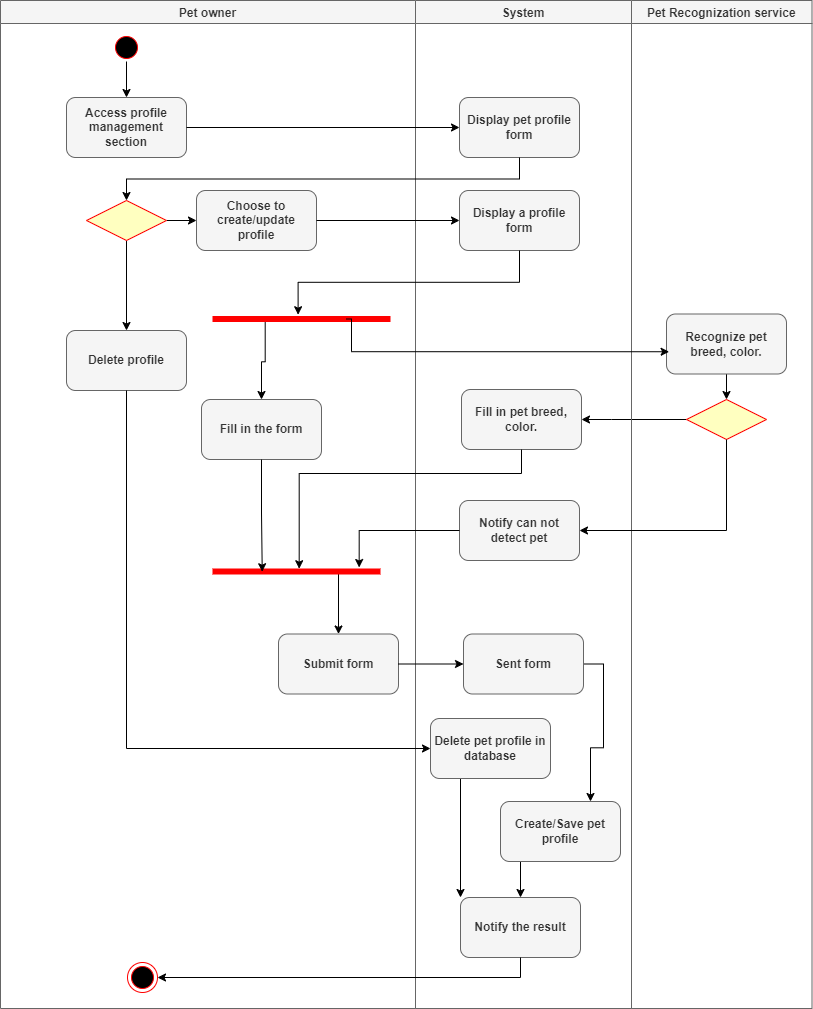
\includegraphics[width=0.7\textwidth]{Figures/manage_pet.png}
  \caption{Manage pet profile activity diagram}
  \label{fig:manage-pet}
\end{figure}

\textbf{Access pet profile}

In the pet profile page, a user has options to find pets by filtering by categories or providing pet images. In case the user filters by images, those images will be processed by the Pet Recognition Service. Then, the filtered pet profiles will be displayed to the user. The user can click on pet profiles for further information or continue finding other pet profiles.

\begin{figure}[H]
  \centering
  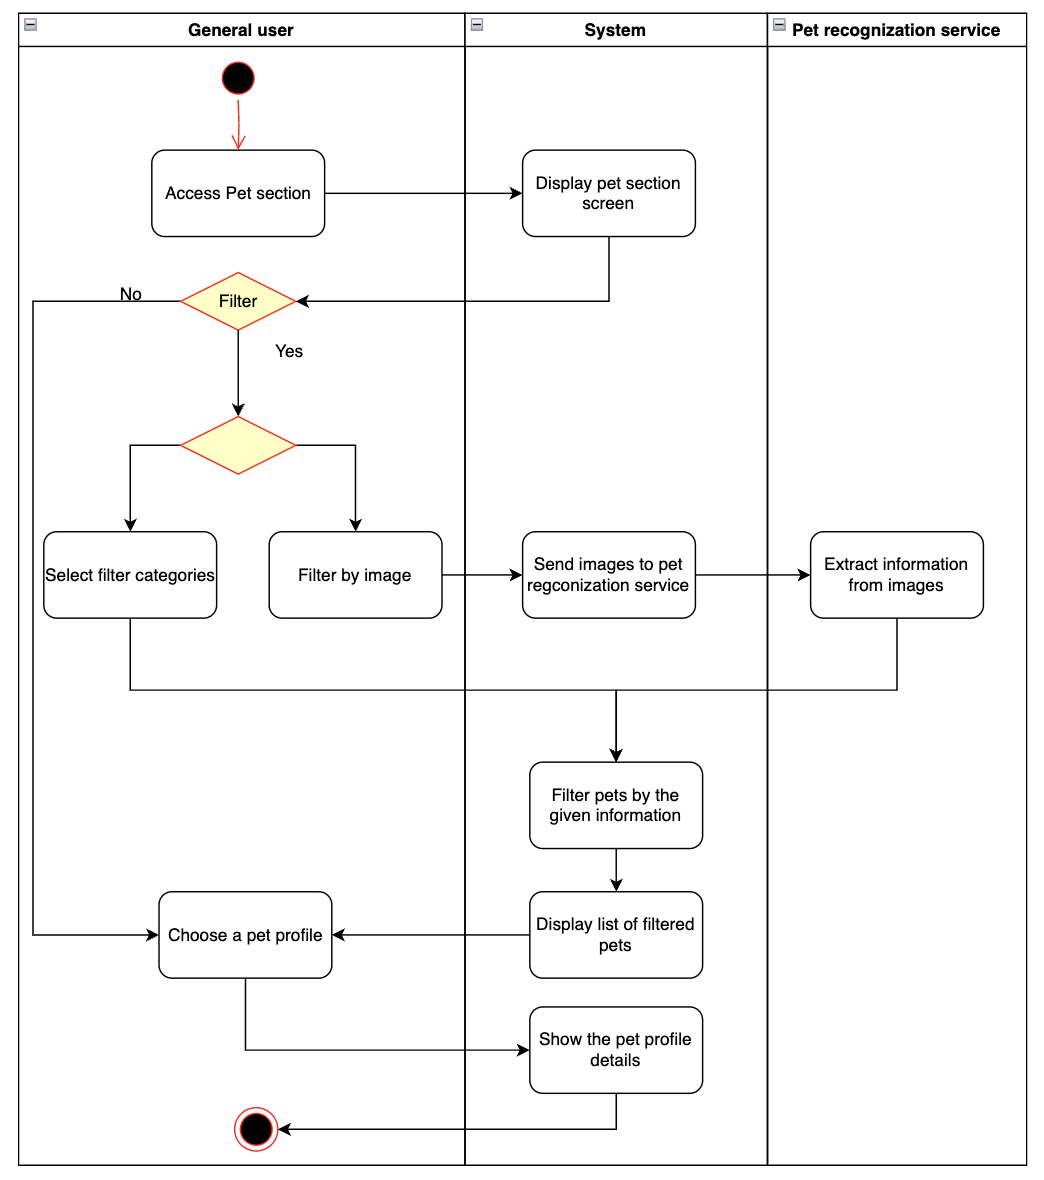
\includegraphics[width=0.7\textwidth]{Figures/access_pet.png}
  \caption{Access pet profile activity diagram}
  \label{fig:access-pet}
\end{figure}

\textbf{Adopt pets}

After finding a pet profile successfully, if the pet is still available, a user can choose to adopt the pet by filling in the required information in the adoption form and sending it. The application form will be reviewed by the pet owner. The result will be sent to the user then. Note that, the user can still contact directly to the pet owner during the pet adoption process.

\begin{figure}[H]
  \centering
  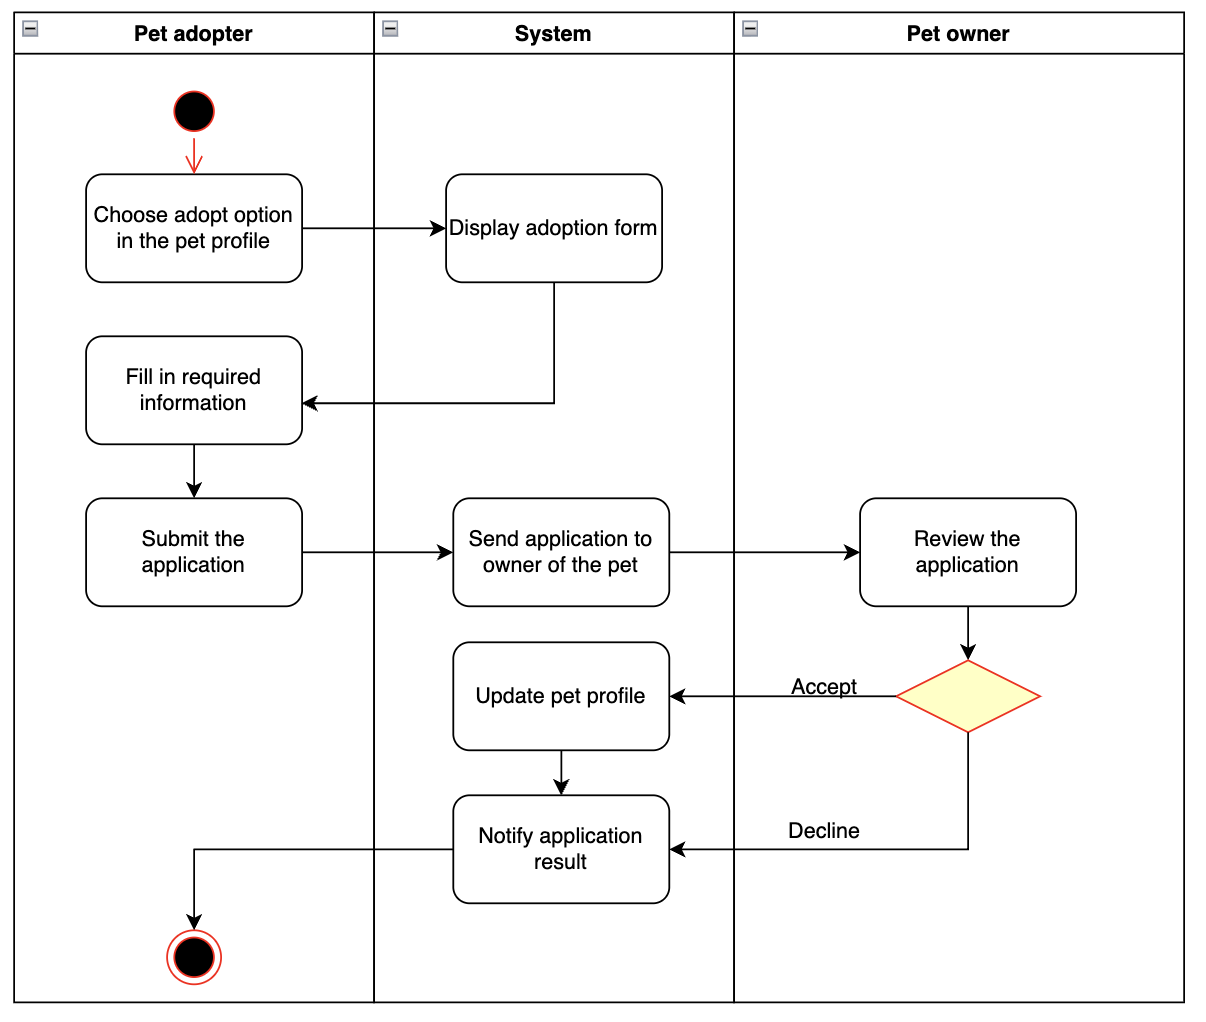
\includegraphics[width=0.7\textwidth]{Figures/adopt_pet.png}
  \caption{Adopt pets activity diagram}
  \label{fig:adopt-pet}
\end{figure}

\textbf{Interact with posts}

After accessing a pet profile successfully, a user can also see public posts of the pet. The user can choose a post for further information and leave their comments or likes on the post. Note that the private posts can only be seen by the pet owner and admins.

\begin{figure}[H]
  \centering
  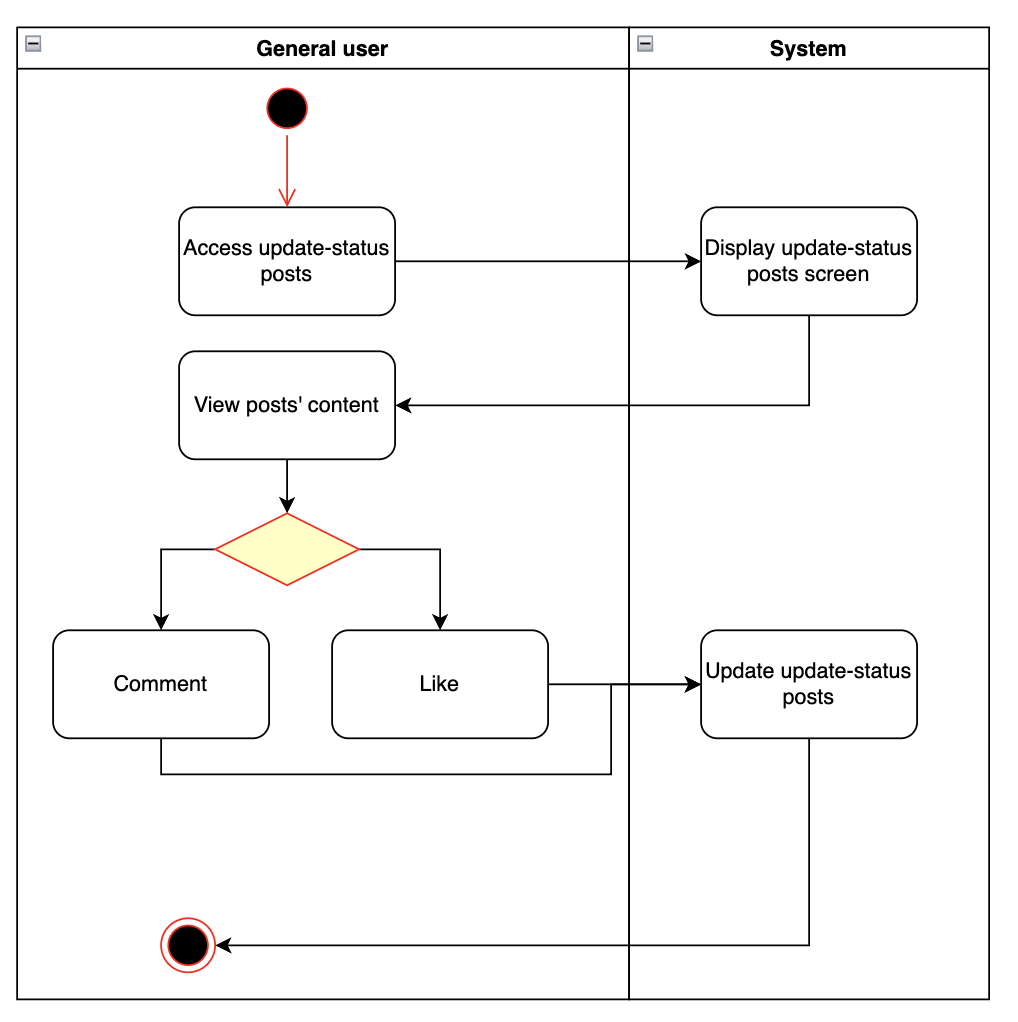
\includegraphics[width=0.7\textwidth]{Figures/post_interact.png}
  \caption{Interact with posts activity diagram}
  \label{fig:interact-post}
\end{figure}


\textbf{Update pet status}

Updating the status of a pet is uploading posts about it. The use case starts when an owner can select a pet profile and choose the option of updating the pet status. After filling information, the owner can set visibility for the post. Finally, the user can send the form and a new post is created.

\begin{figure}[H]
  \centering
  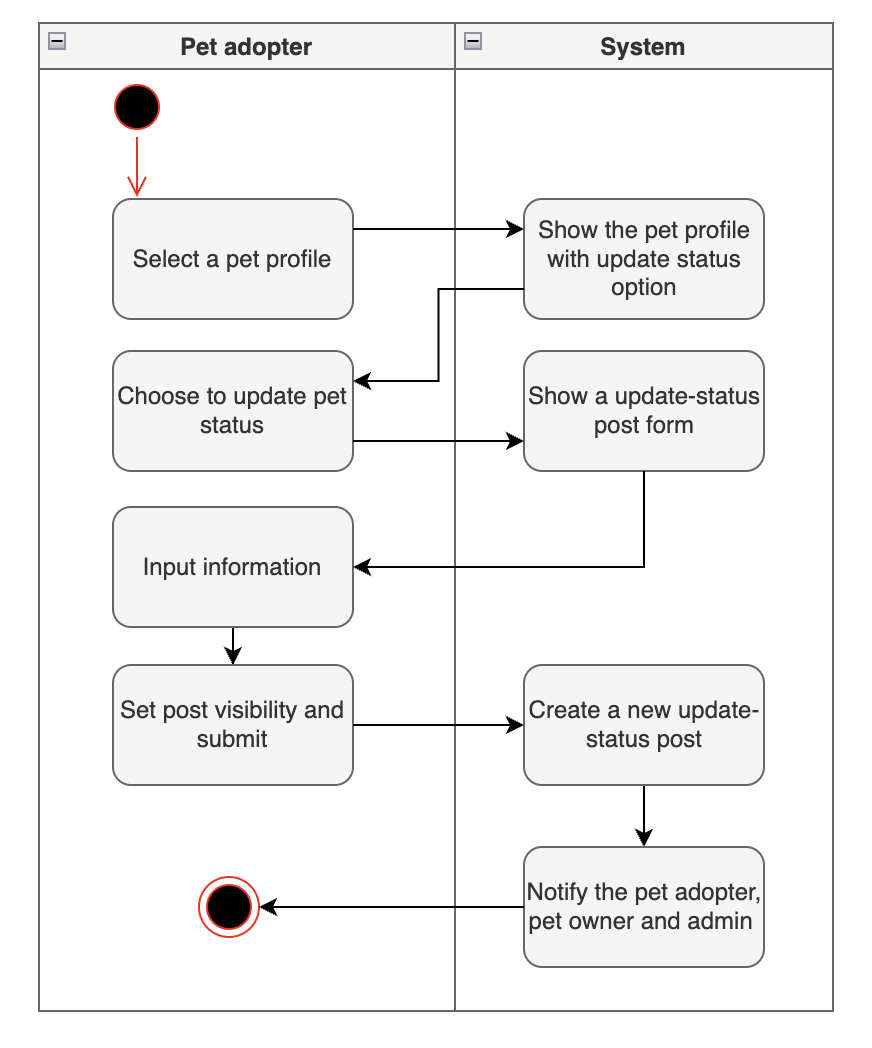
\includegraphics[width=0.7\textwidth]{Figures/pet_status.png}
  \caption{Update pet status activity diagram}
  \label{fig:update-pet-status}
\end{figure}

\textbf{Manage blogs for Organizations}

The use case starts when a user with an Organization account accesses the blog management page. The user chooses to edit or create a new blog, then a form will be displayed. Note that the form would be filled if the user chose to edit an available blog. In that case, the user can modify the fields or rather delete the blog. If the user wants to create a new blog, the user can input and submit it. Finally, admins will verify the blog and the result will be sent to the user.

\begin {figure}[H]
\centering
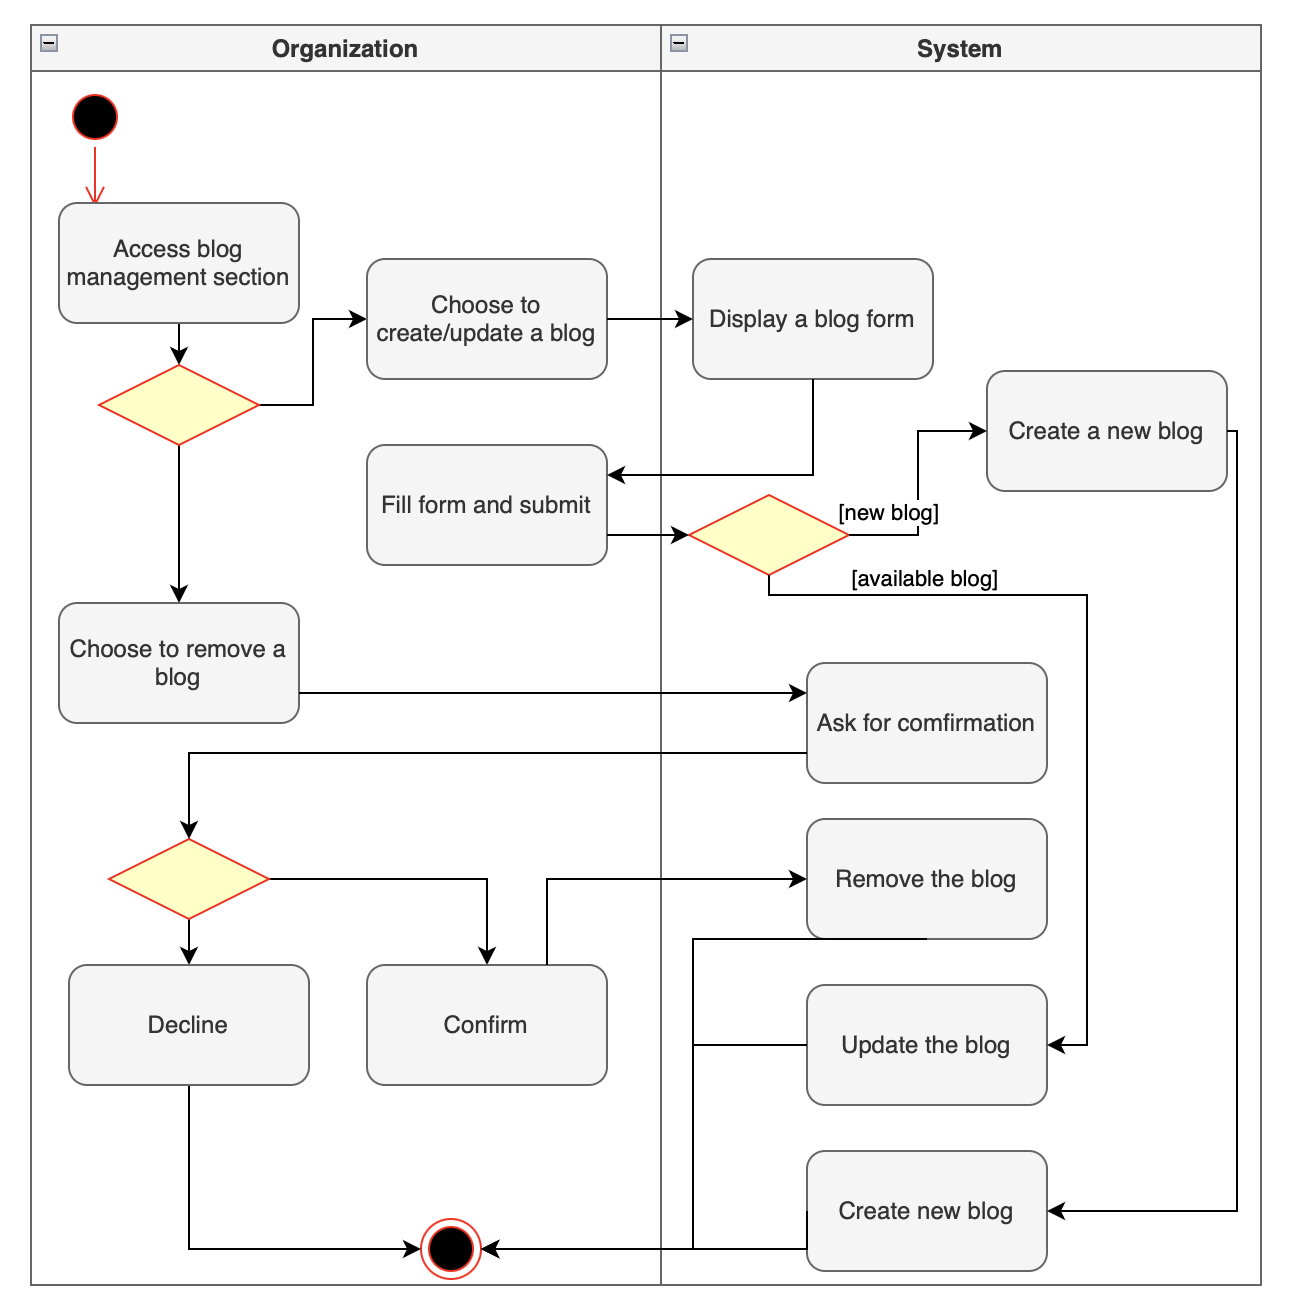
\includegraphics[width=0.7\textwidth]{Figures/manage_blog_org.png}
\caption{Manage blogs for Organizations activity diagram}
\label{fig:manage-blog}
\end{figure}

\textbf{Manage blogs for Administrator}

The use case starts when a user with an Organization account accesses the blog management page. The flow is almost the same as for Organization users except that the blog is created without any verification.

\begin {figure}[H]
\centering
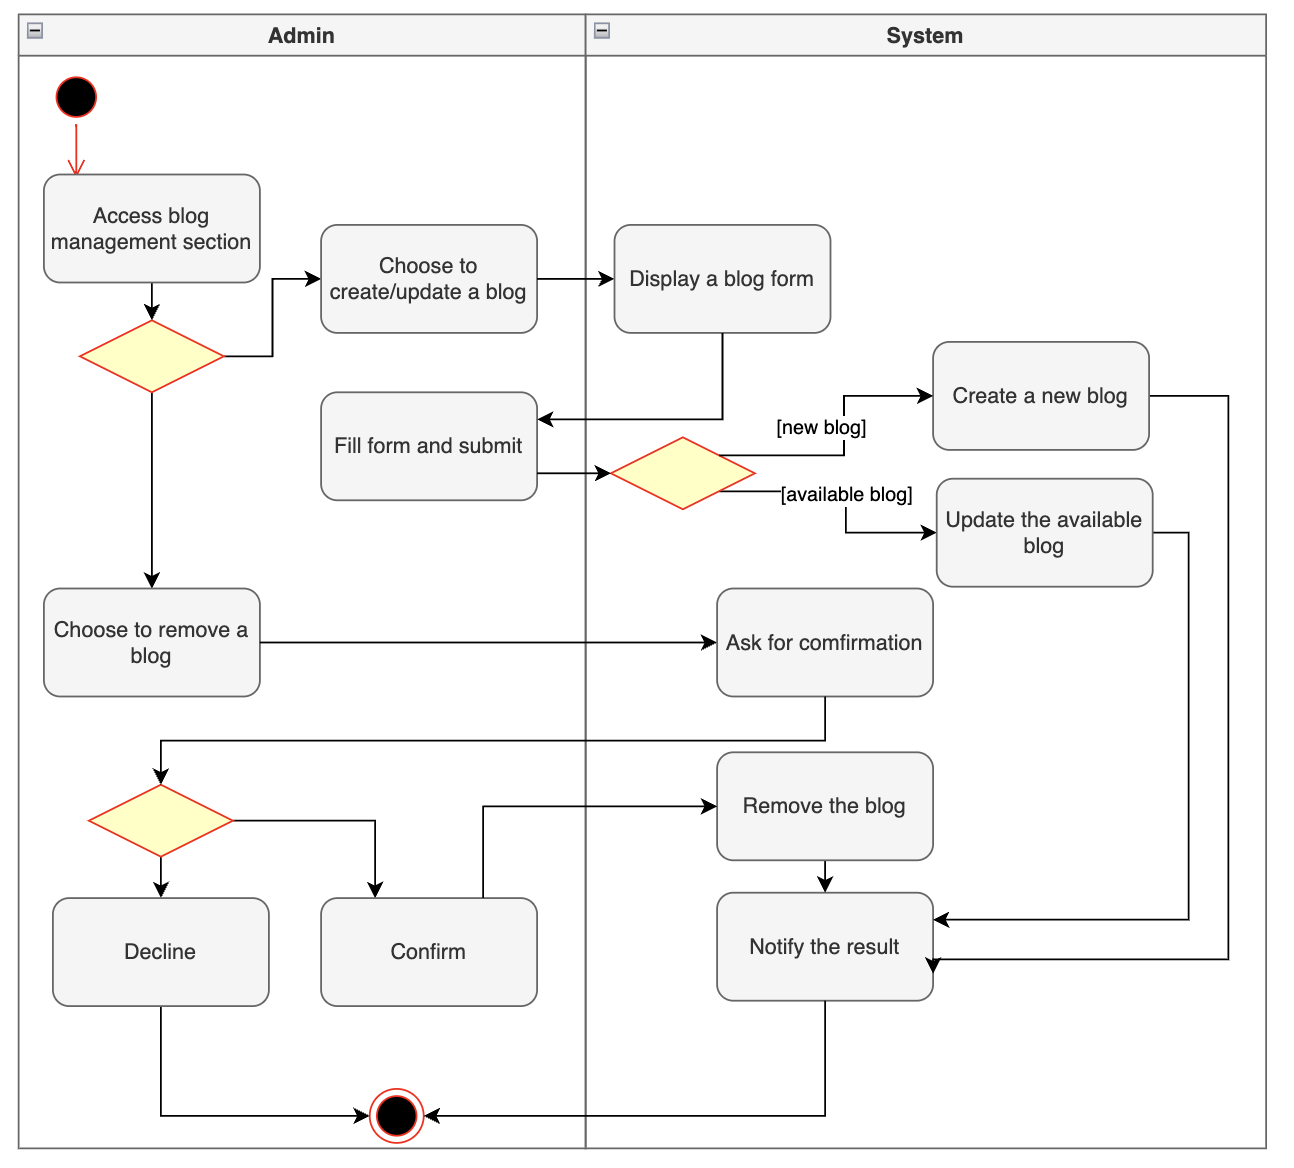
\includegraphics[width=0.7\textwidth]{Figures/manage_blog_admin.png}
\caption{Manage blogs for Administrator activity diagram}
\label{fig:manage-blog-admin}
\end{figure}

\textbf{Make payment}

When a user applies an advertisement on a log, the system shows all advertisement types with their periods. Then, users choose a type of advertisement and the system shows the payment invoice. If the user confirms the payment, the Payment service will process the transaction and the result will be displayed to admins and the user.

\begin {figure}[H]
\centering
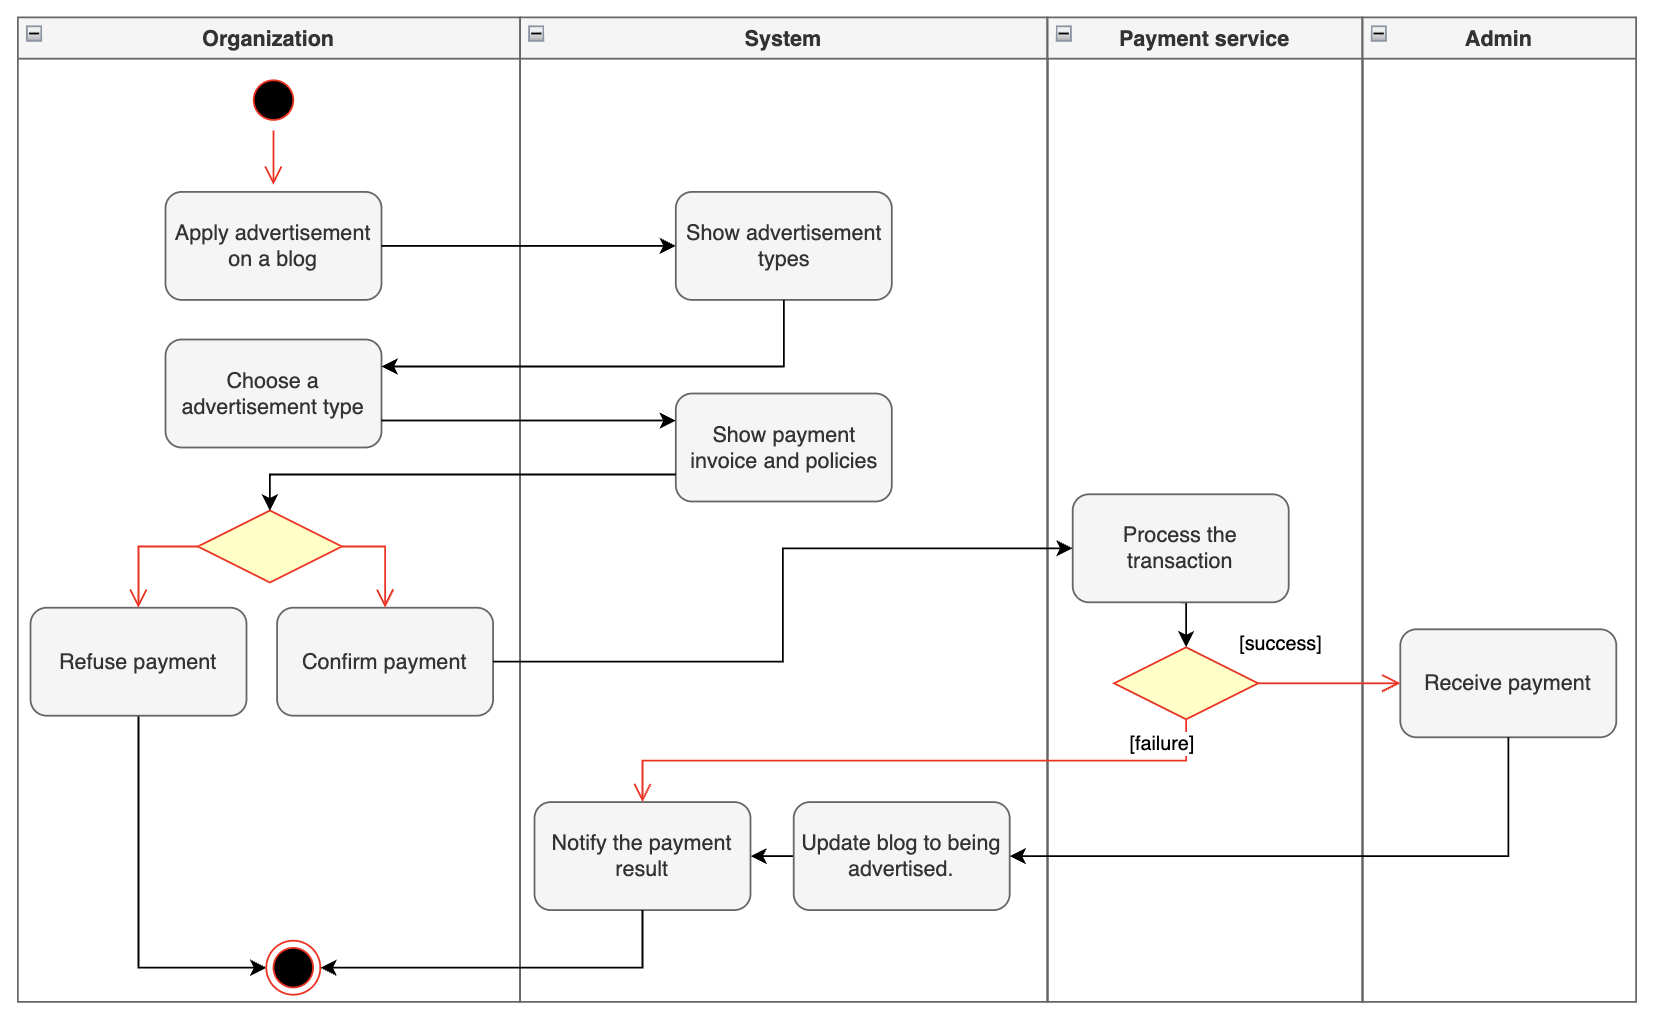
\includegraphics[width=0.7\textwidth]{Figures/payment.png}
\caption{Make payment activity diagram}
\label{fig:make-payment}
\end{figure}

\subsection{Class Diagrams}

The system design is expected to adhere to the Layered and Repository
design patterns as outlined in \emph{\textbf{section 3.1}}.
Consequently, the system's classes are categorized into four distinct
groups.

\emph{View Classes} (Figure 21): These classes encompass the user
interface and user experience (UI/UX) components, along with methods for
handling user events. Each class inherits from a common class,
\emph{BaseLayout}, which encapsulates the components and methods shared
across all view classes.

\emph{Service Classes} (Figure 22): These classes contain methods for
processing the system's logic and business flow. Each class has a
specific responsibility and inherits from a class called
\emph{BaseService}, which encapsulates the methods and services common
to all service classes. The methods of service classes are made
available to view classes via an Application Programming Interface
(API).

\emph{DataLayer Classes} (Figure 23): Each class corresponds to a system
entity in the database. All DataLayer classes inherit from a class
called \emph{BaseDataLayer}, which provides all the methods needed to
interact with the database. It's important to note that a DataLayer
class can only interact with its corresponding entity in the database.

\emph{UnitOfWork} Class (Figure 23): This singular class contains
properties that are instances of DataLayer classes. The BaseService
class implements the UnitOfWork, enabling all service classes to access
the database. This class also includes methods to save changes or
rollback transactions in case of any exceptions at the end of an
application process.

This structure ensures a clear separation of concerns, promoting
maintainability and scalability in the system design.

\begin{figure}[H]
  \centering
  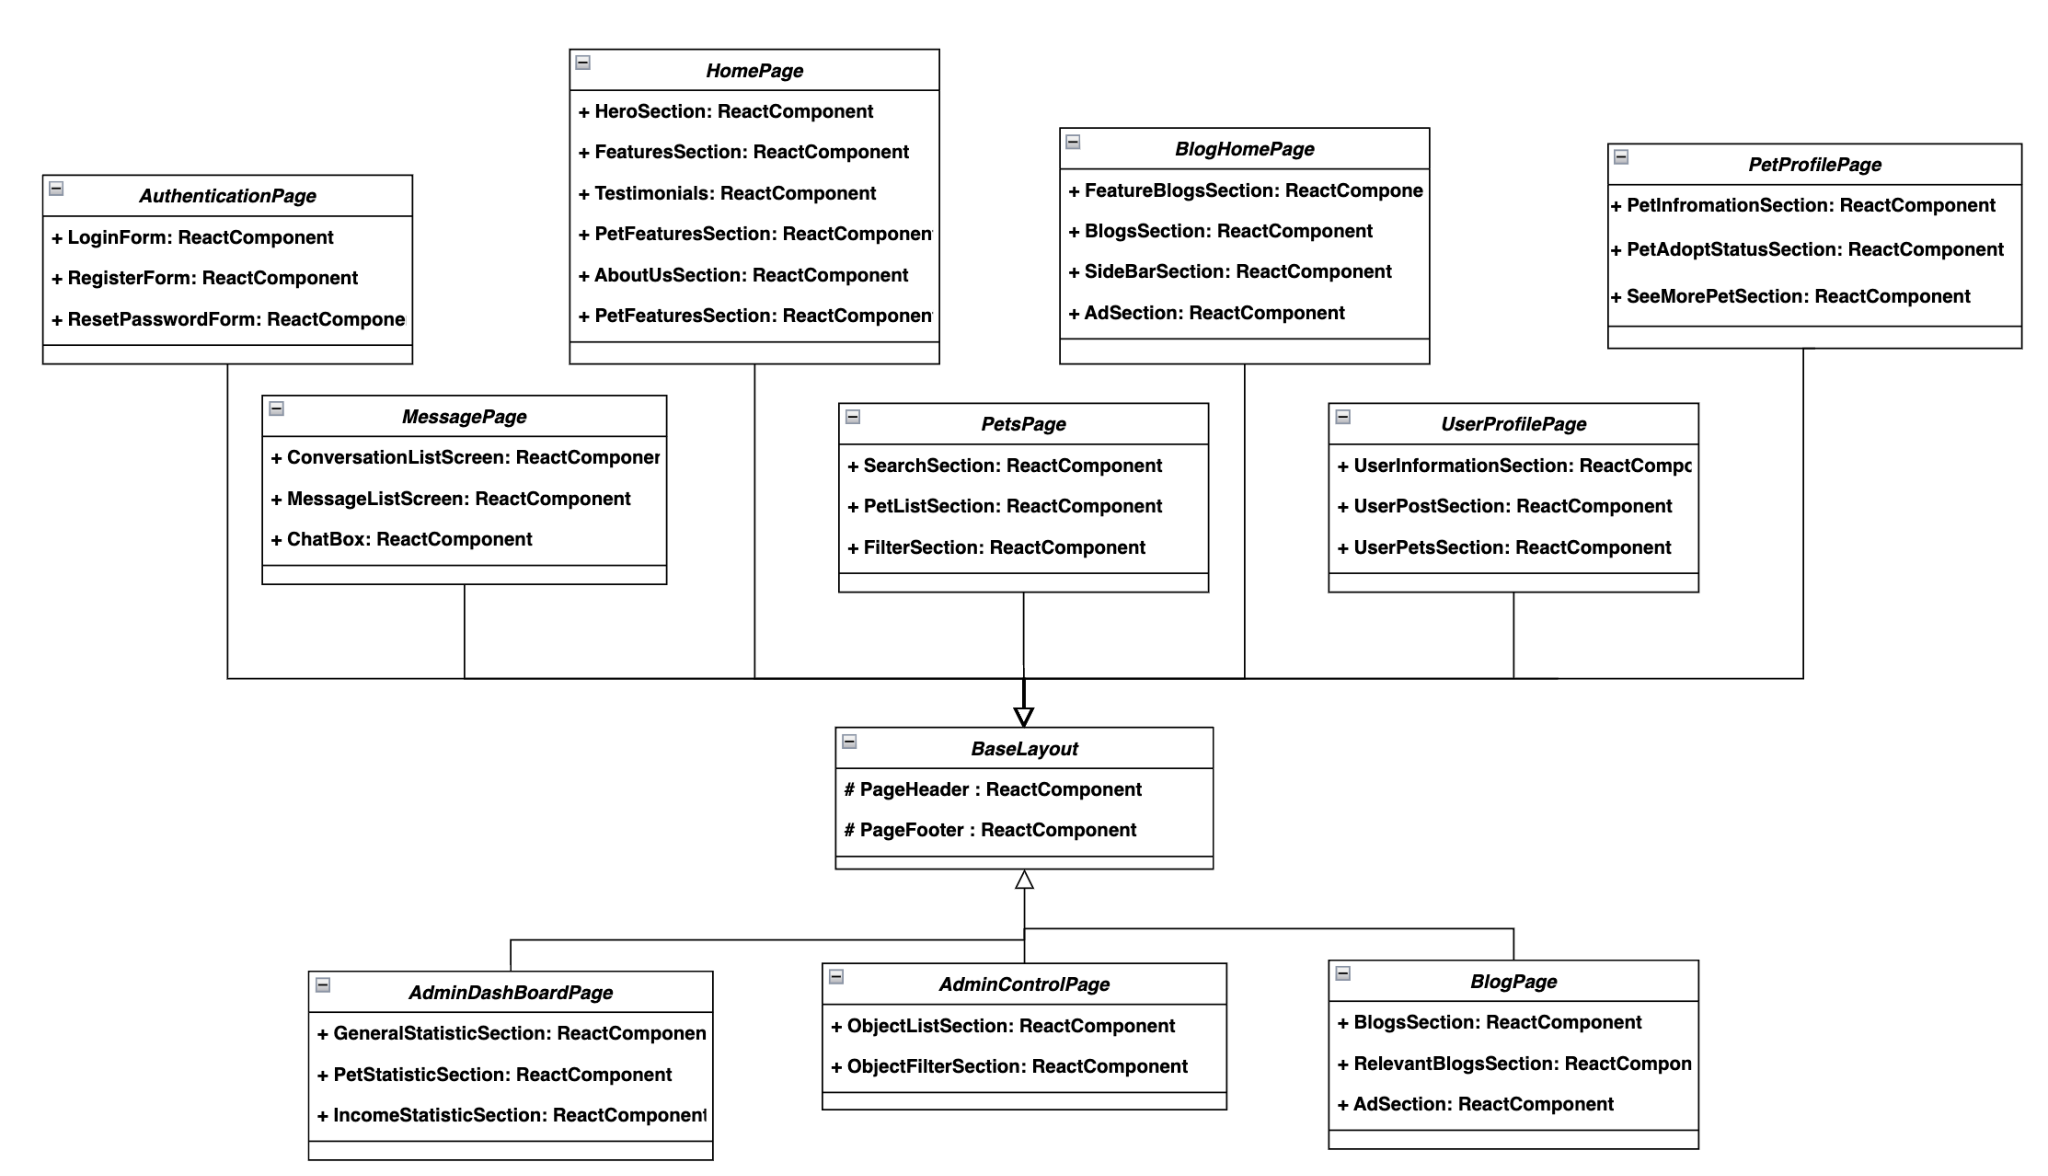
\includegraphics[angle=-90,width=0.8\textwidth]{Figures/view_class.png}
  \caption{View Classes}
  \label{fig:view-classes}
\end{figure}
\clearpage

\begin{figure}[H]
  \centering
  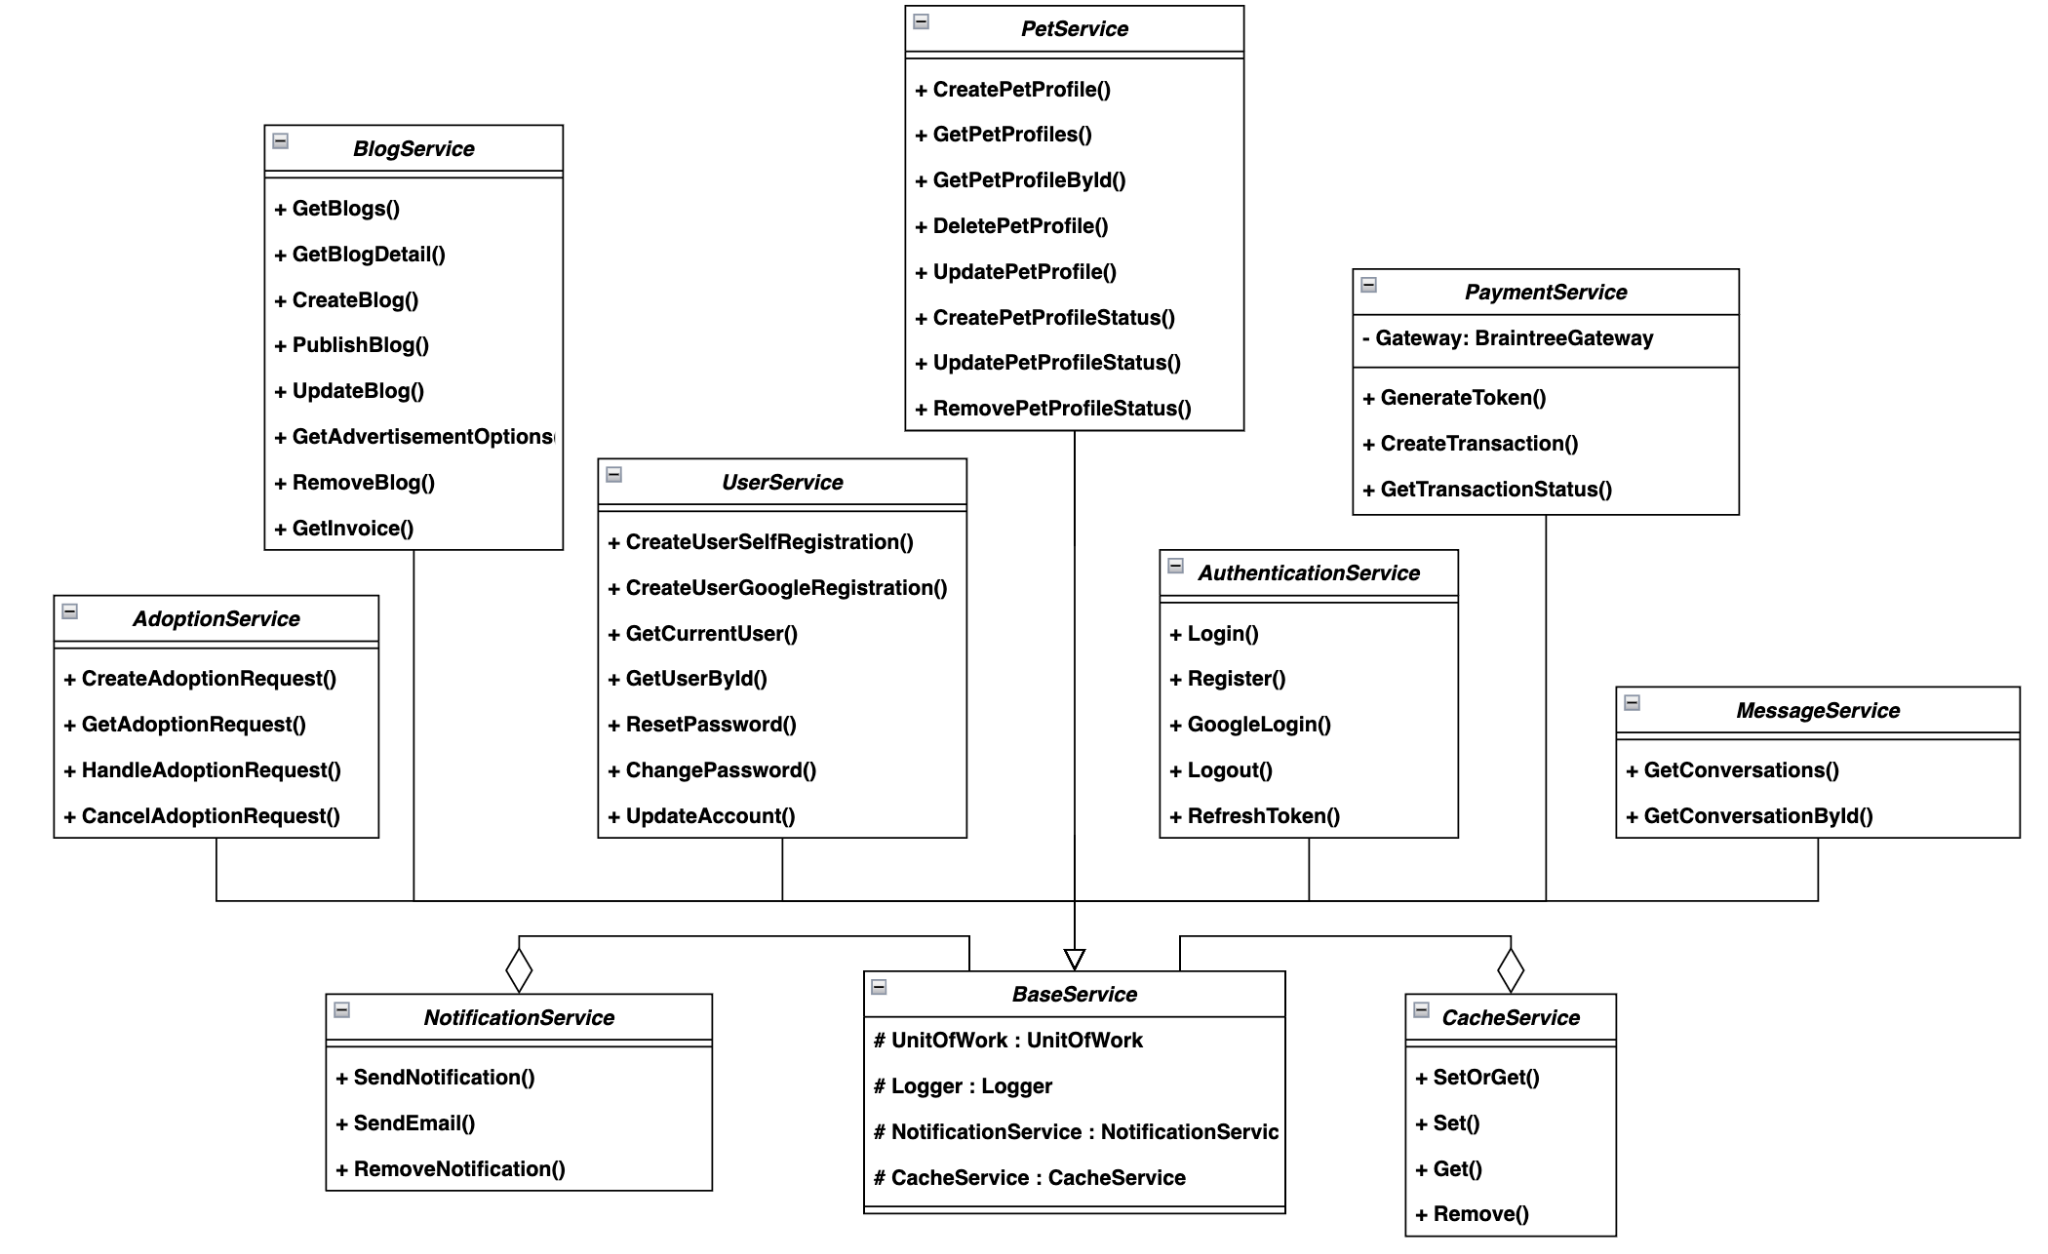
\includegraphics[angle=-90,width=0.8\textwidth]{Figures/service_class.png}
  \caption{Service Classes}
  \label{fig:service-classes}
\end{figure}

\begin{figure}[H]
  \centering
  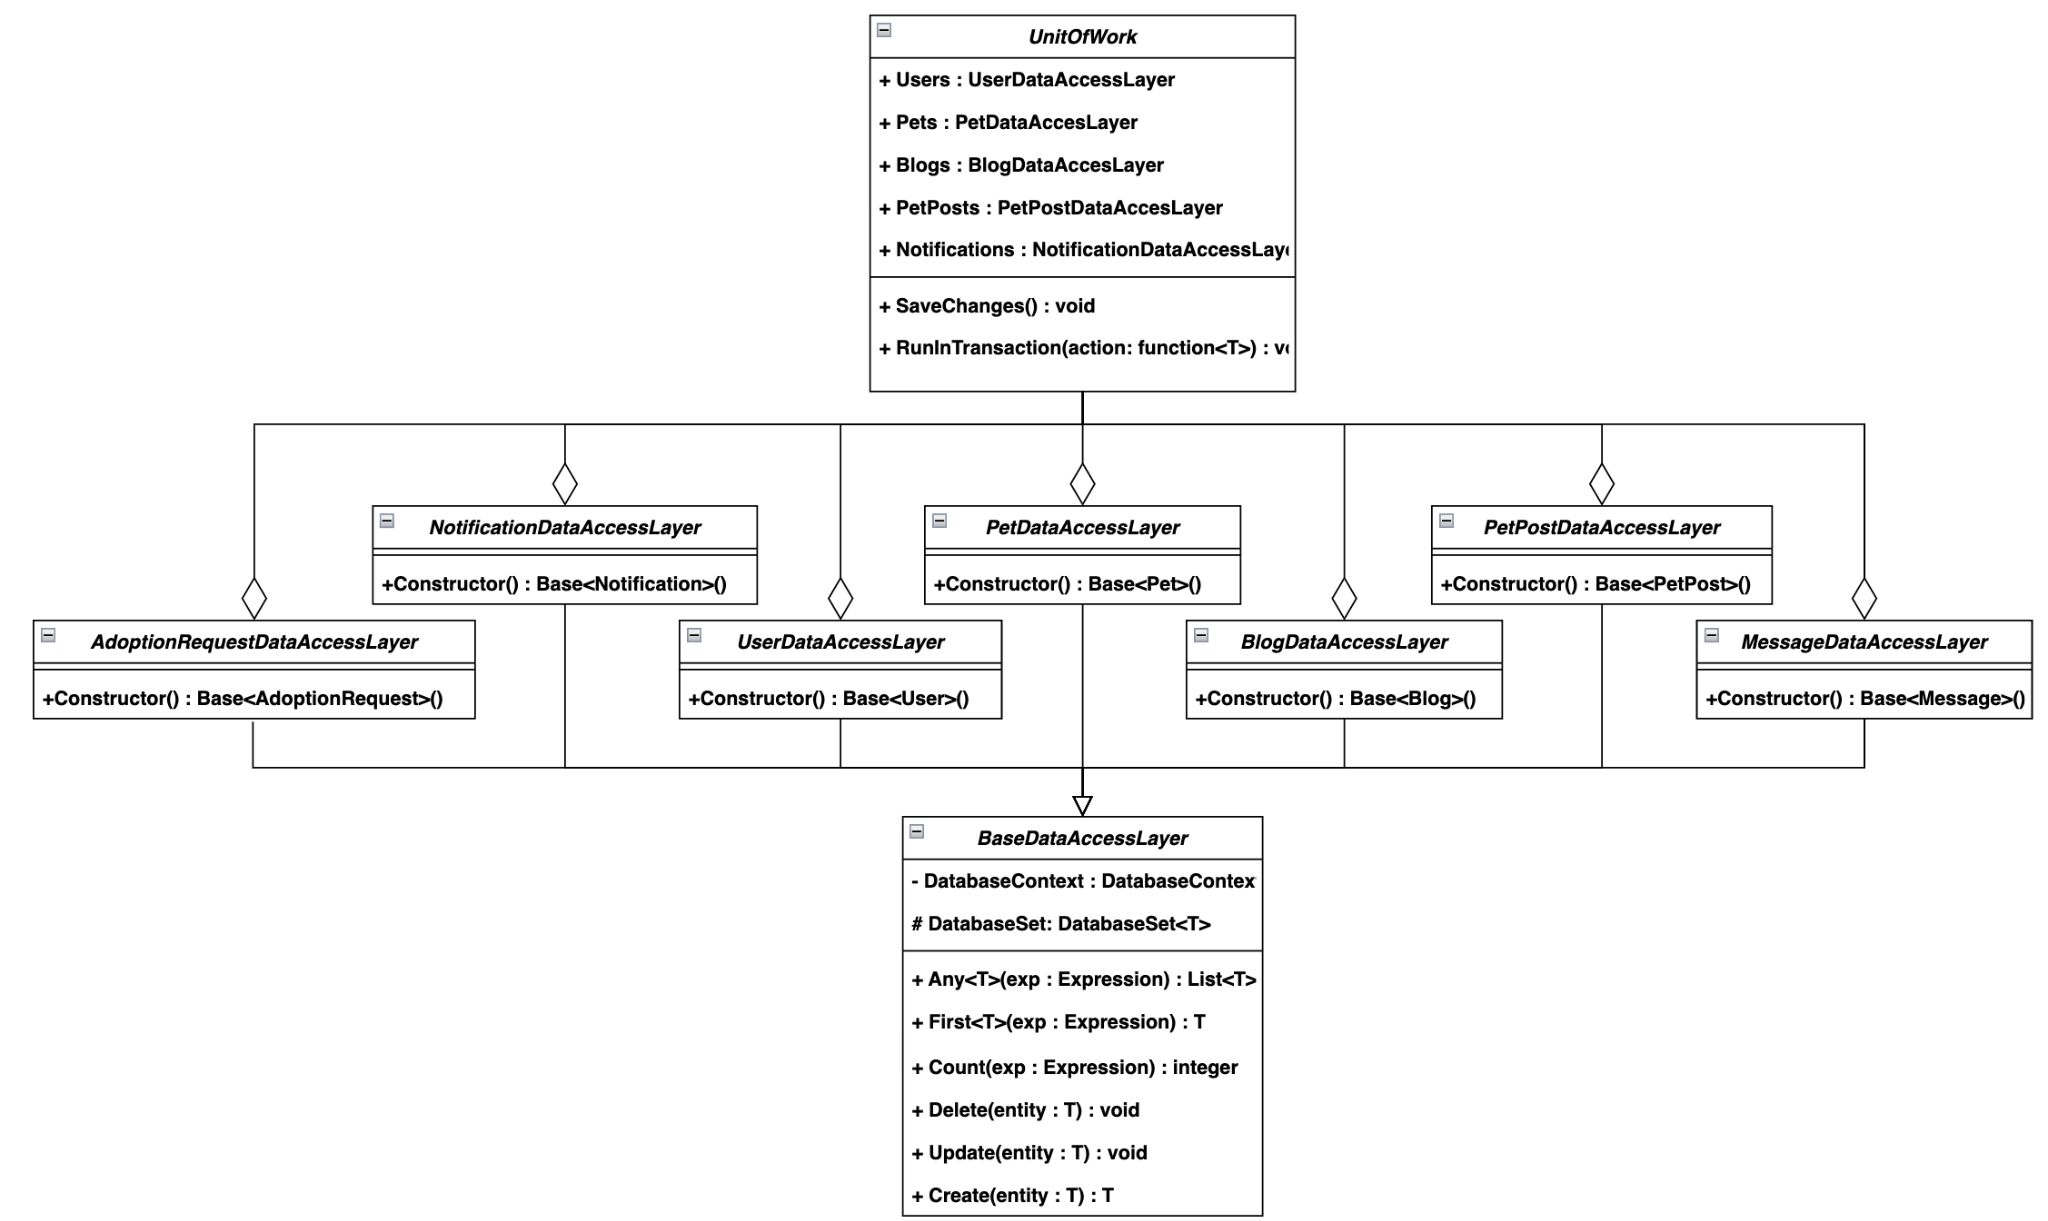
\includegraphics[angle=-90,width=0.8\textwidth]{Figures/uow_class.png}
  \caption{DataLayer Classes}
  \label{fig:datalayer-classes}
\end{figure}
\clearpage

\subsection{Sequence Diagrams}

After completing the class diagrams and activity diagrams of the system, we will  demonstrate how the system's classes interact with each other according to the system's business flow using sequence diagrams.

\textbf{Self Registration}

\begin{figure}[H]
  \centering
  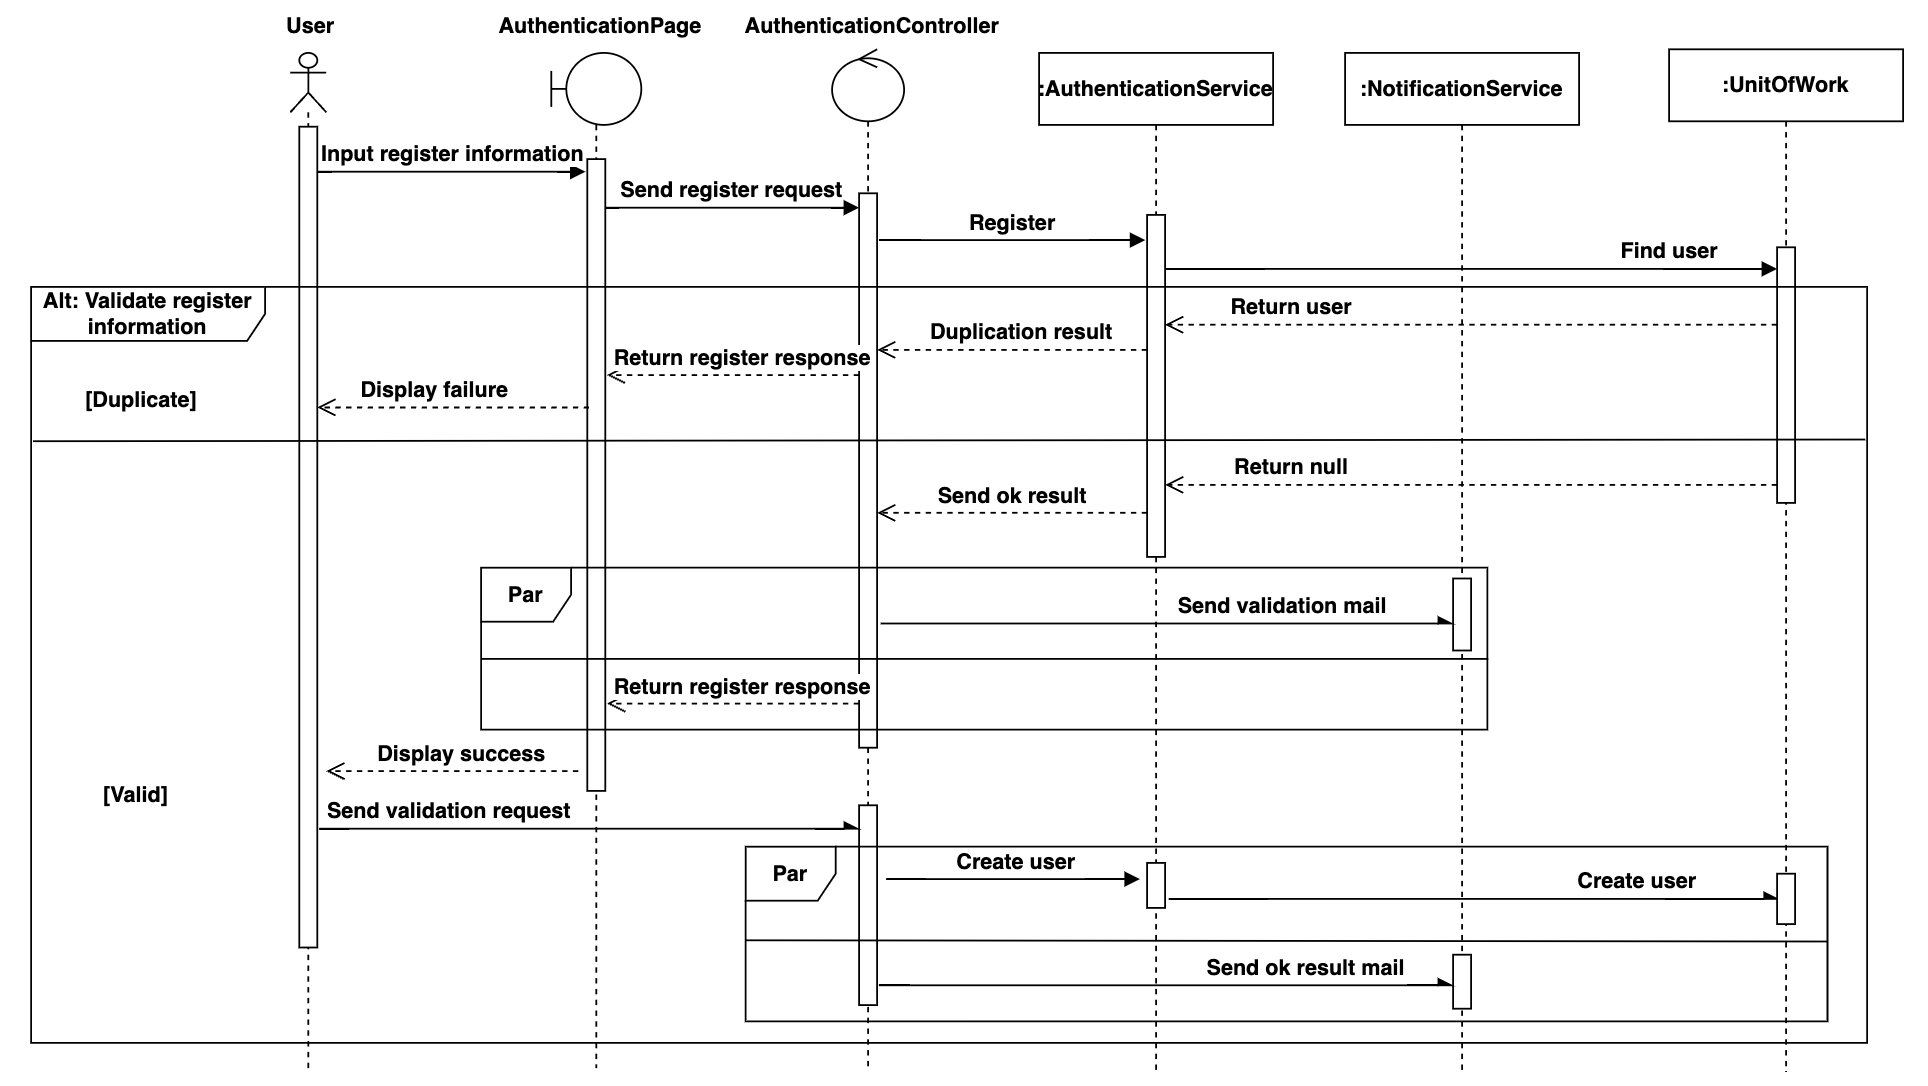
\includegraphics[width=0.9\textwidth]{Figures/self_register_seq.png}
  \caption{Self Registration sequence diagram}
  \label{fig:self-registration-seq}
\end{figure}


\textbf{Login}

\begin{figure}[H]
  \centering
  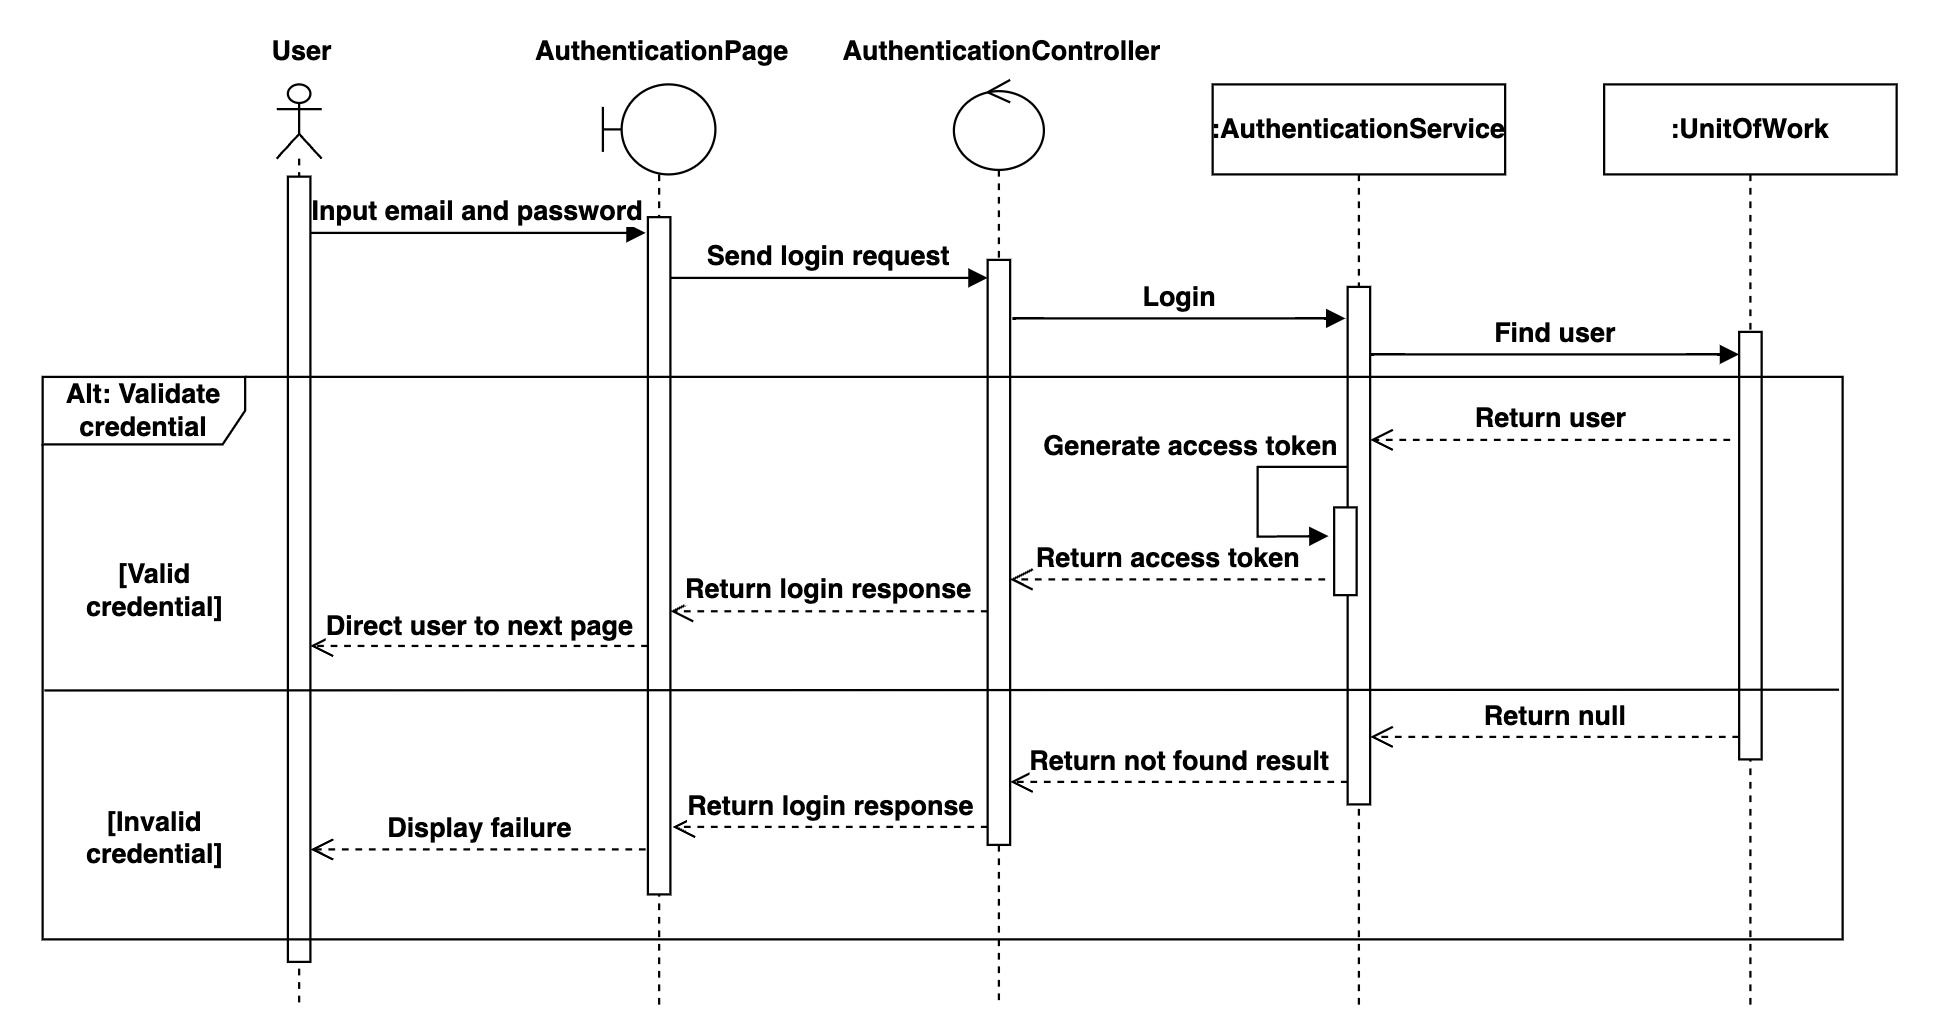
\includegraphics[width=0.9\textwidth]{Figures/login_seq.png}
  \caption{Login sequence diagram}
  \label{fig:login-seq}
\end{figure}
\clearpage
\textbf{Login with a Google account}

\begin{figure}[H]
  \centering
  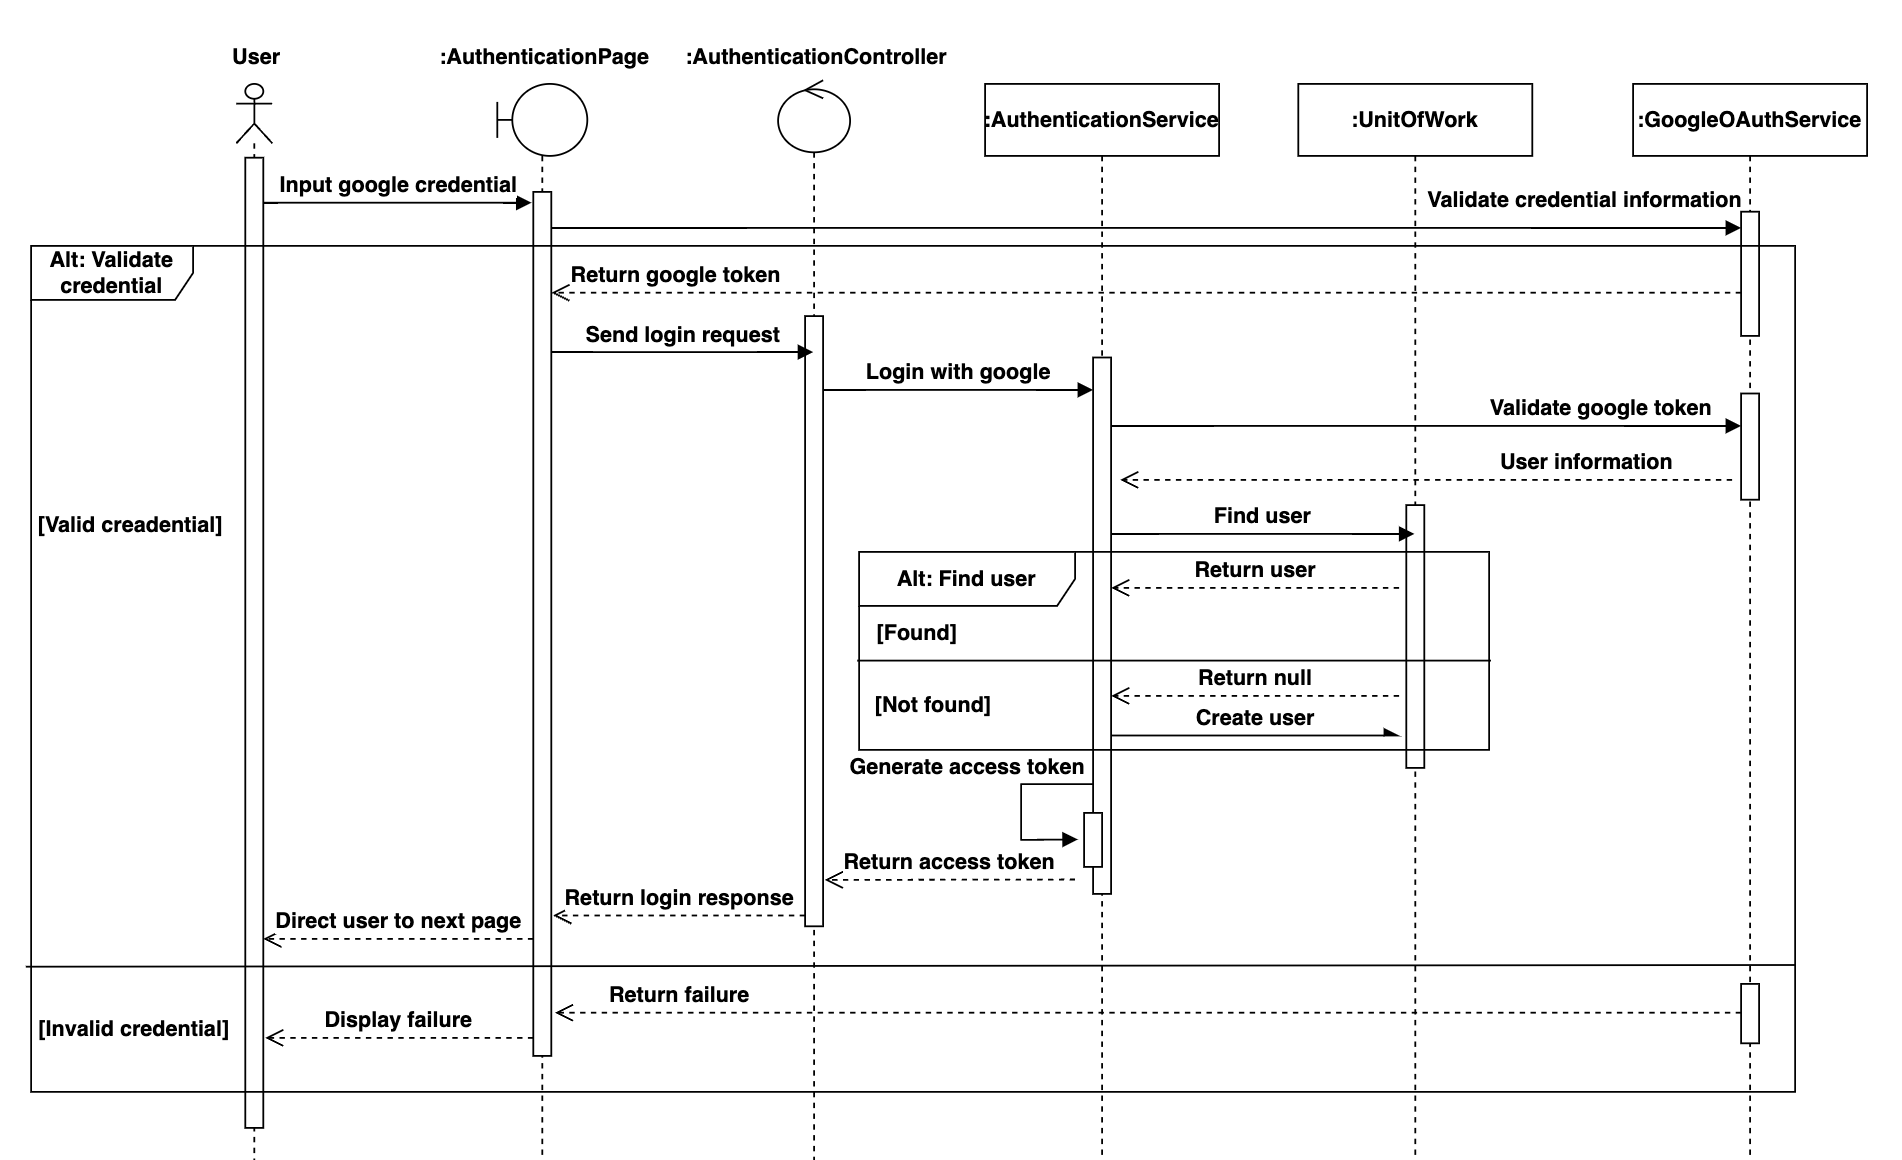
\includegraphics[width=0.9\textwidth]{Figures/login_gg_seq.png}
  \caption{Login with a Google account sequence diagram}
  \label{fig:login-google-seq}
\end{figure}

\textbf{Update to Organization account}

\begin{figure}[H]
  \centering
  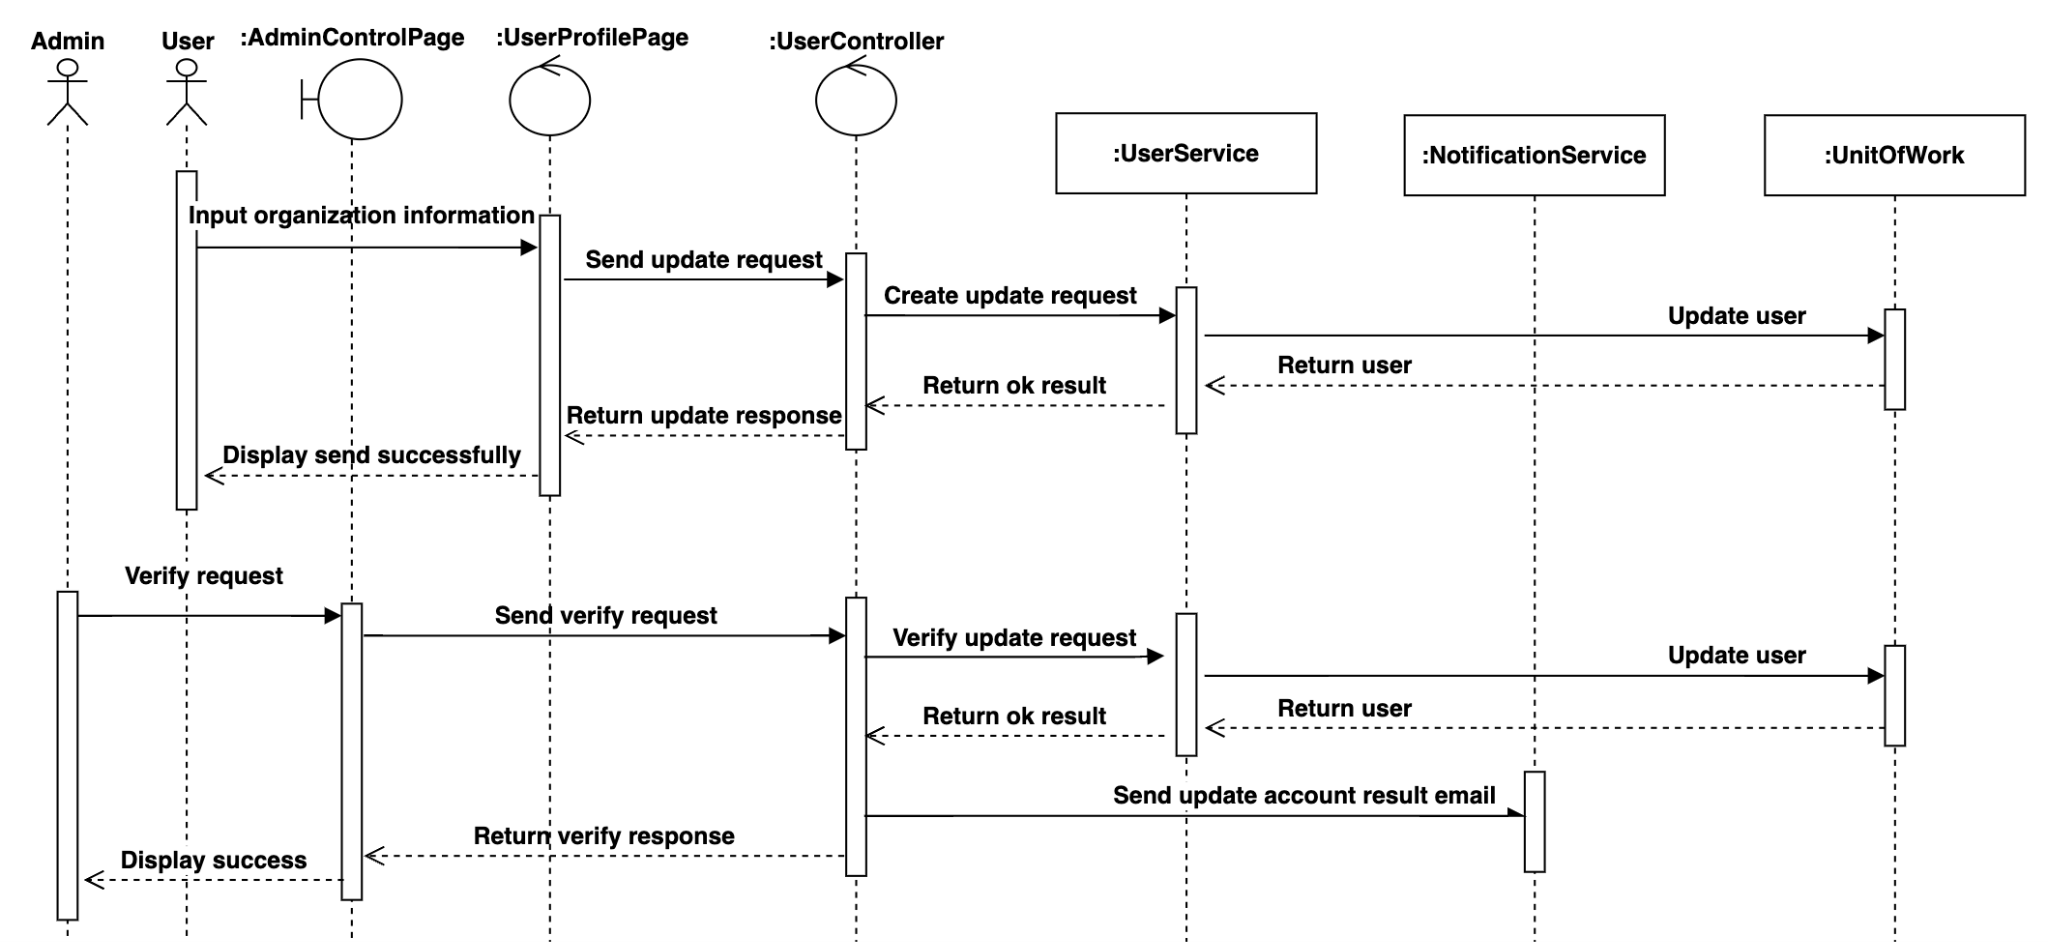
\includegraphics[width=0.9\textwidth]{Figures/update_org_seq.png}
  \caption{Update to Organization account sequence diagram}
  \label{fig:update-org-seq}
\end{figure}

\textbf{Manage pet profile}

\begin{figure}[H]
  \centering
  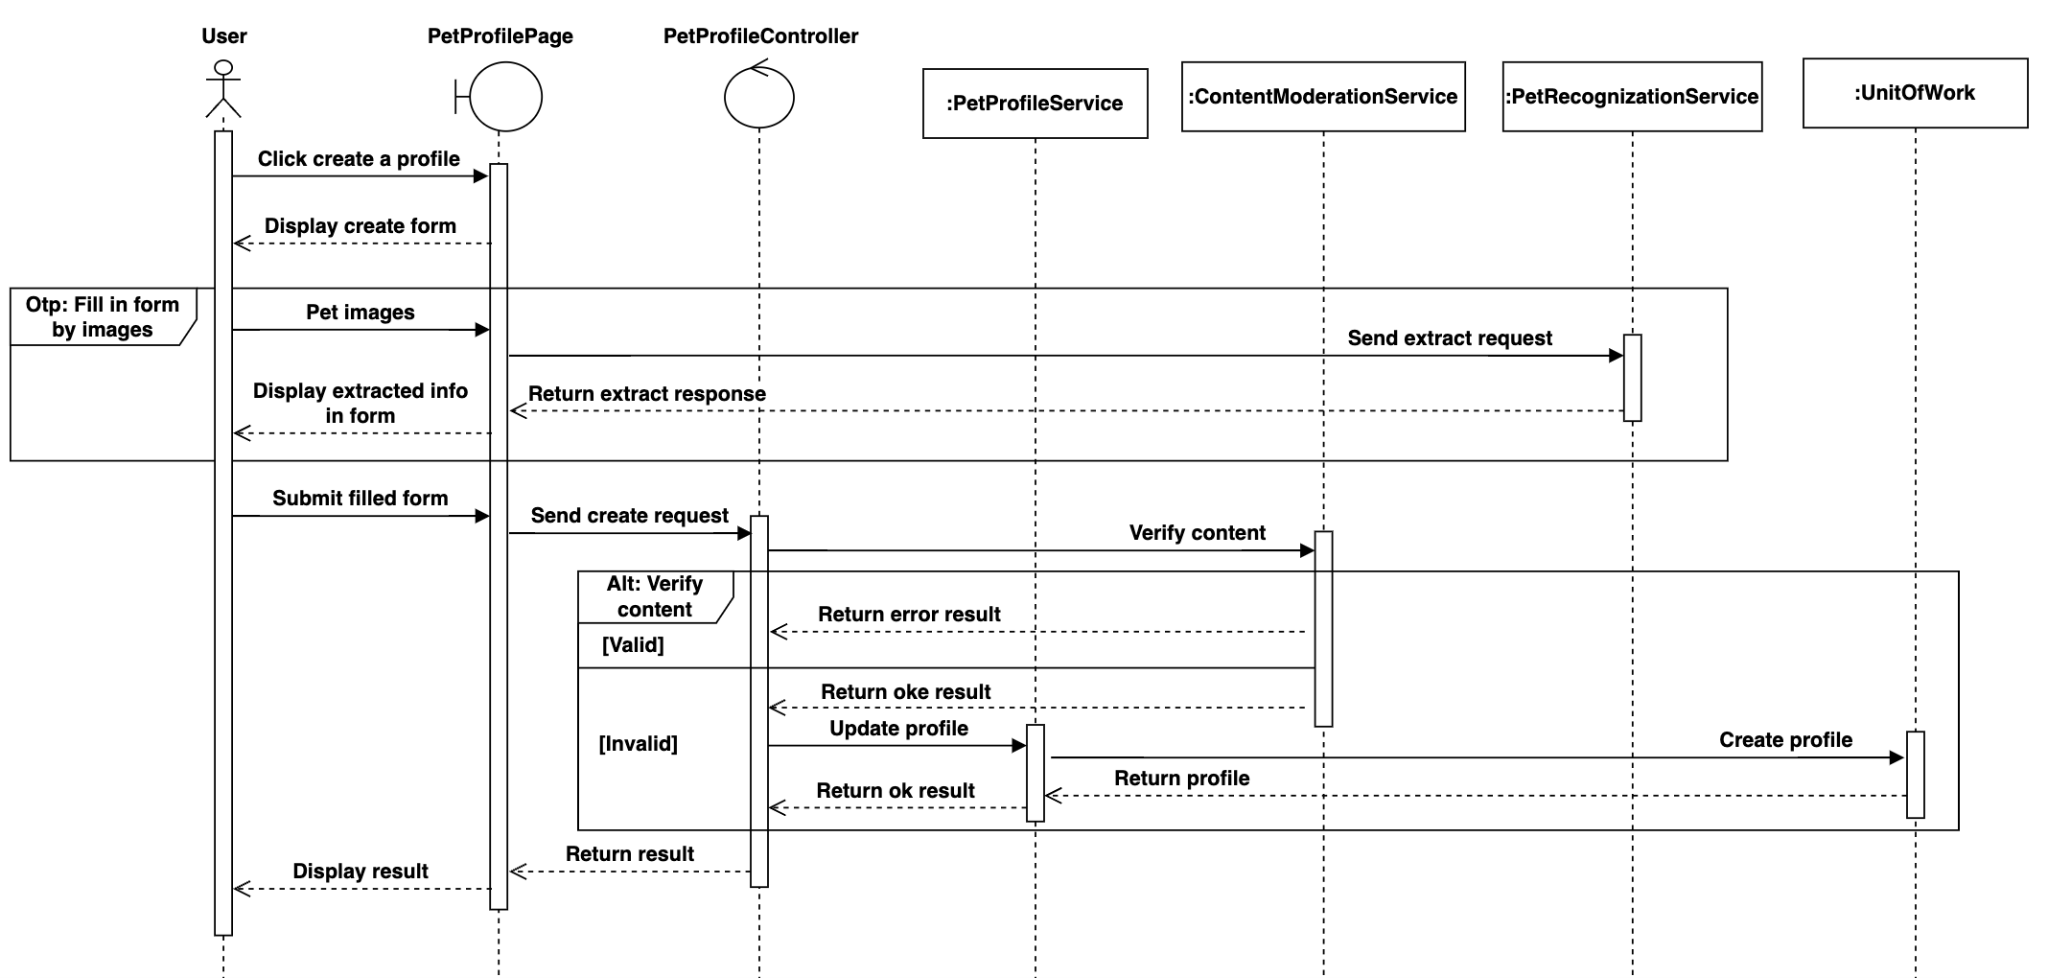
\includegraphics[angle=-90,width=0.7\textwidth]{Figures/manage_pet_seq.png}
  \caption{Create pet profile sequence diagram}
  \label{fig:manage-pet-seq}
\end{figure}
\clearpage
\begin{figure}[H]
  \centering
  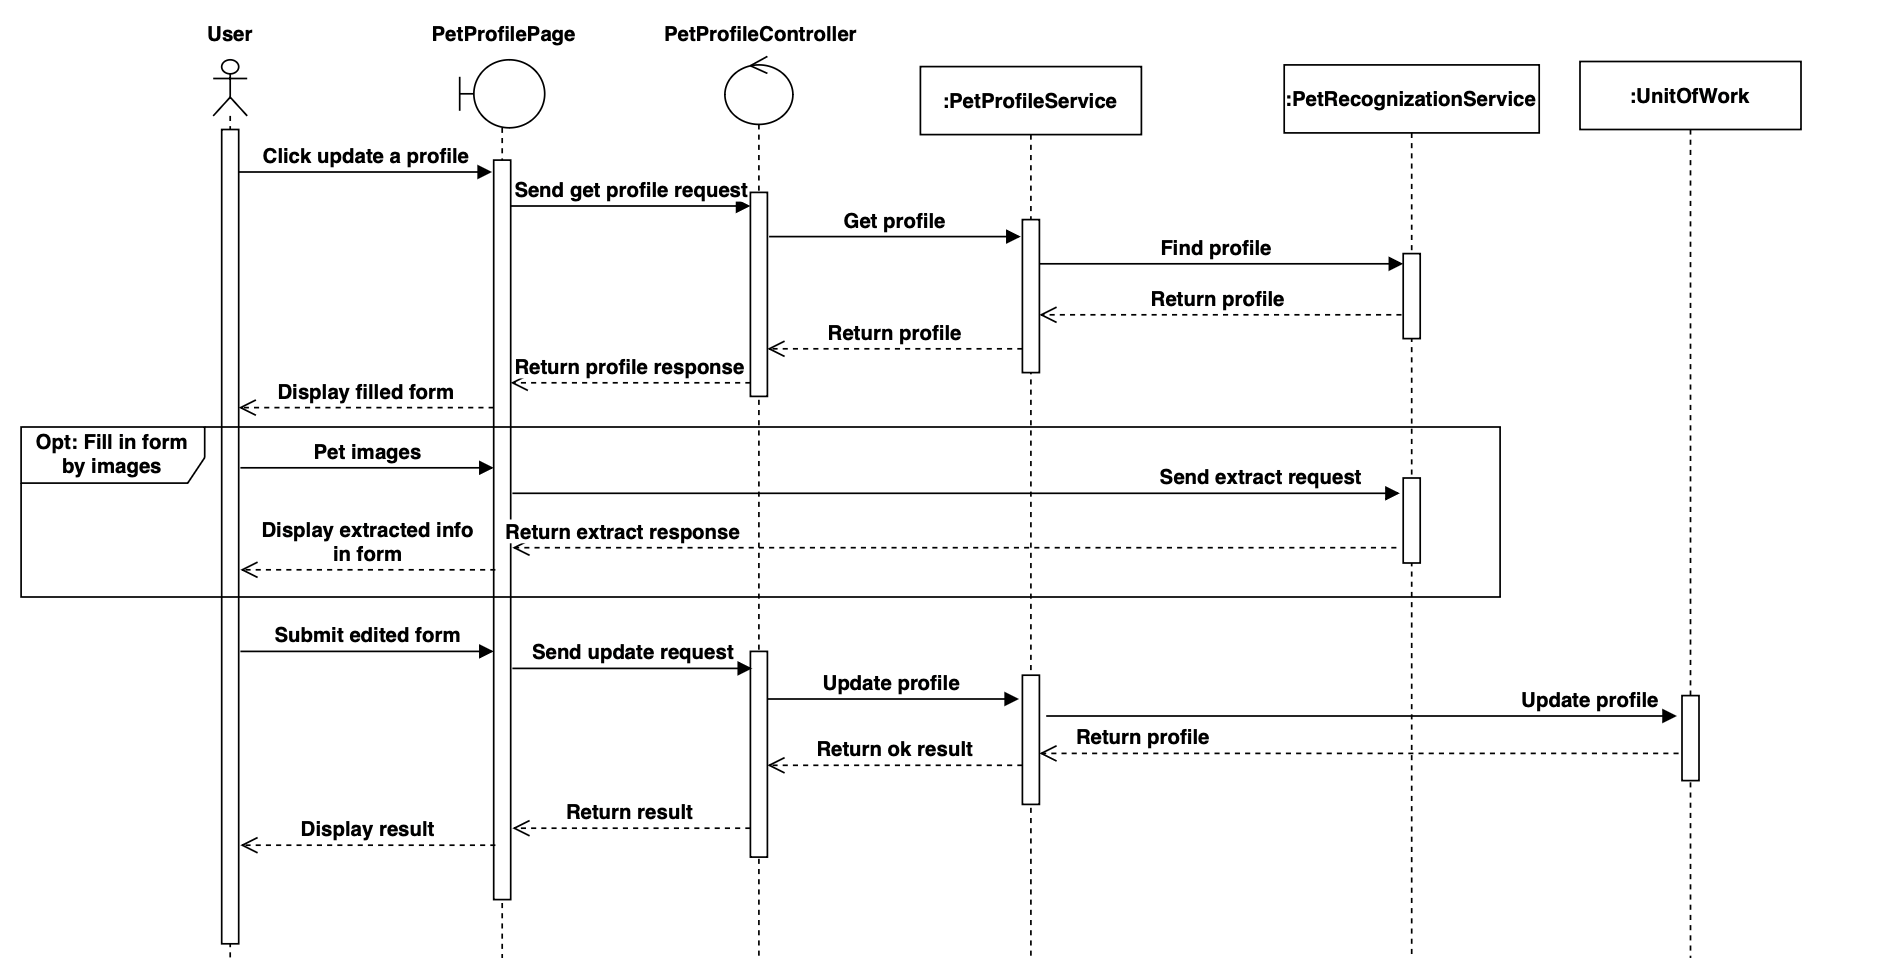
\includegraphics[angle=-90,width=0.7\textwidth]{Figures/update_pet_profile_seq.png}
  \caption{Update pet profile sequence diagram}
  \label{fig:access-pet-seq}
\end{figure}
\clearpage

\textbf{Manage blogs}

\begin{figure}[H]
  \centering
  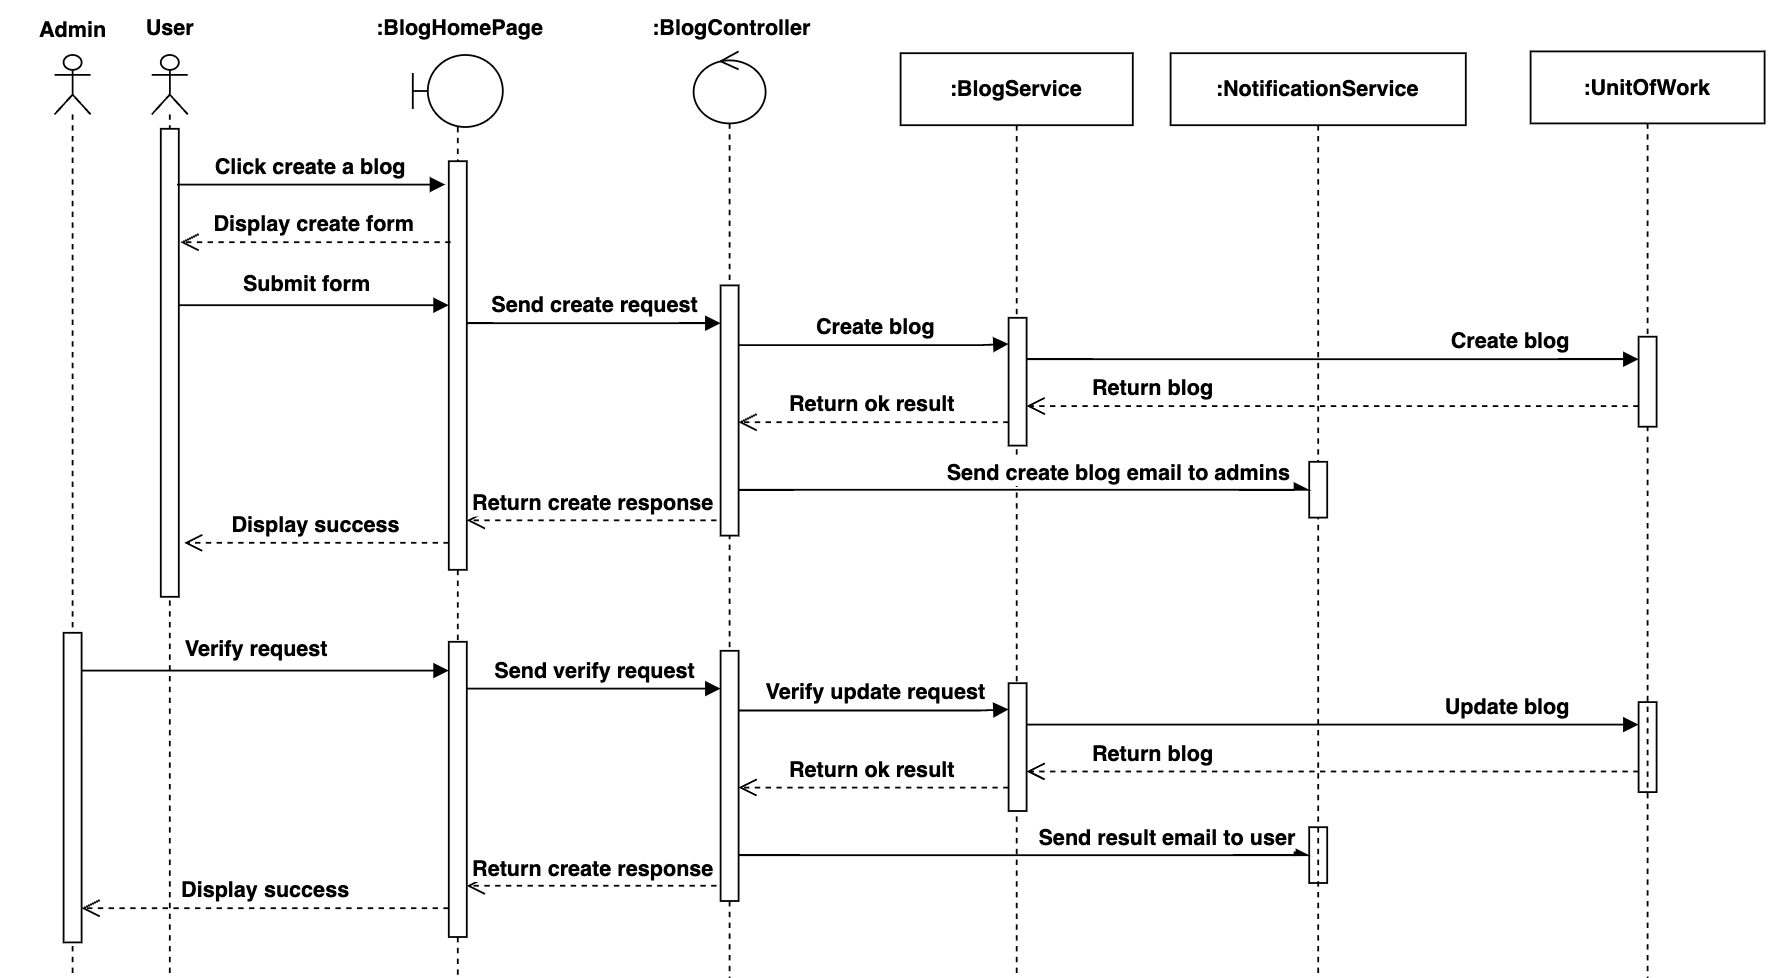
\includegraphics[width=0.9\textwidth]{Figures/manage_blog_seq.png}
  \caption{Create blogs sequence diagram}
  \label{fig:manage-blog-seq}
\end{figure}

\begin{figure}[H]
  \centering
  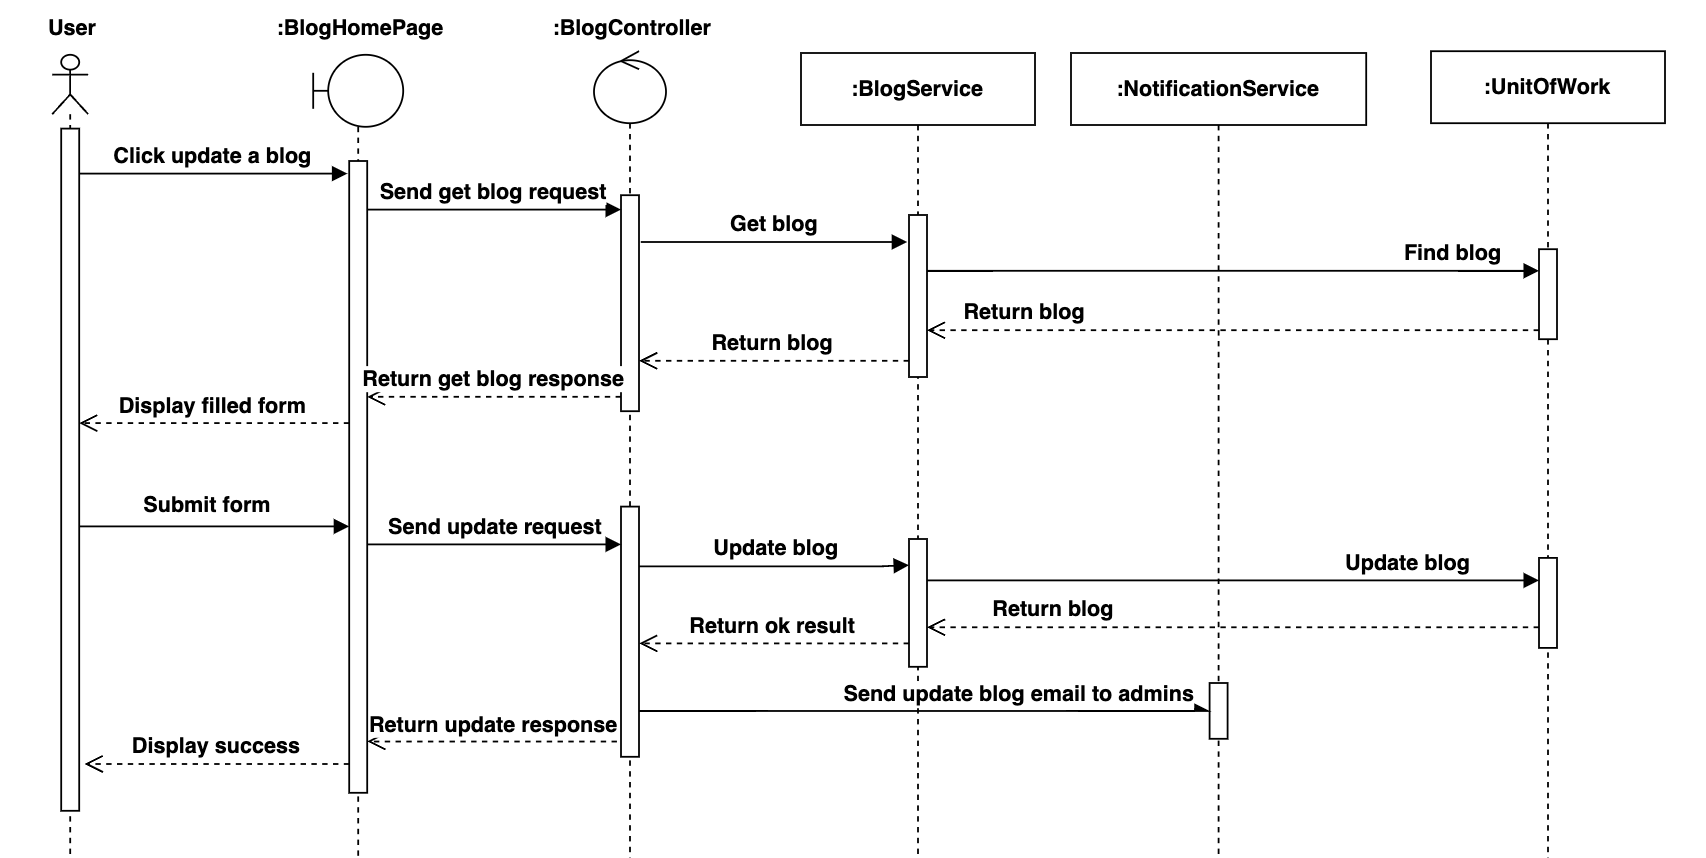
\includegraphics[width=0.9\textwidth]{Figures/update_blog_seq.png}
  \caption{Update blogs sequence diagram}
  \label{fig:update-blog-seq}
\end{figure}
\clearpage
\textbf{Make payment}

\begin{figure}[H]
  \centering
  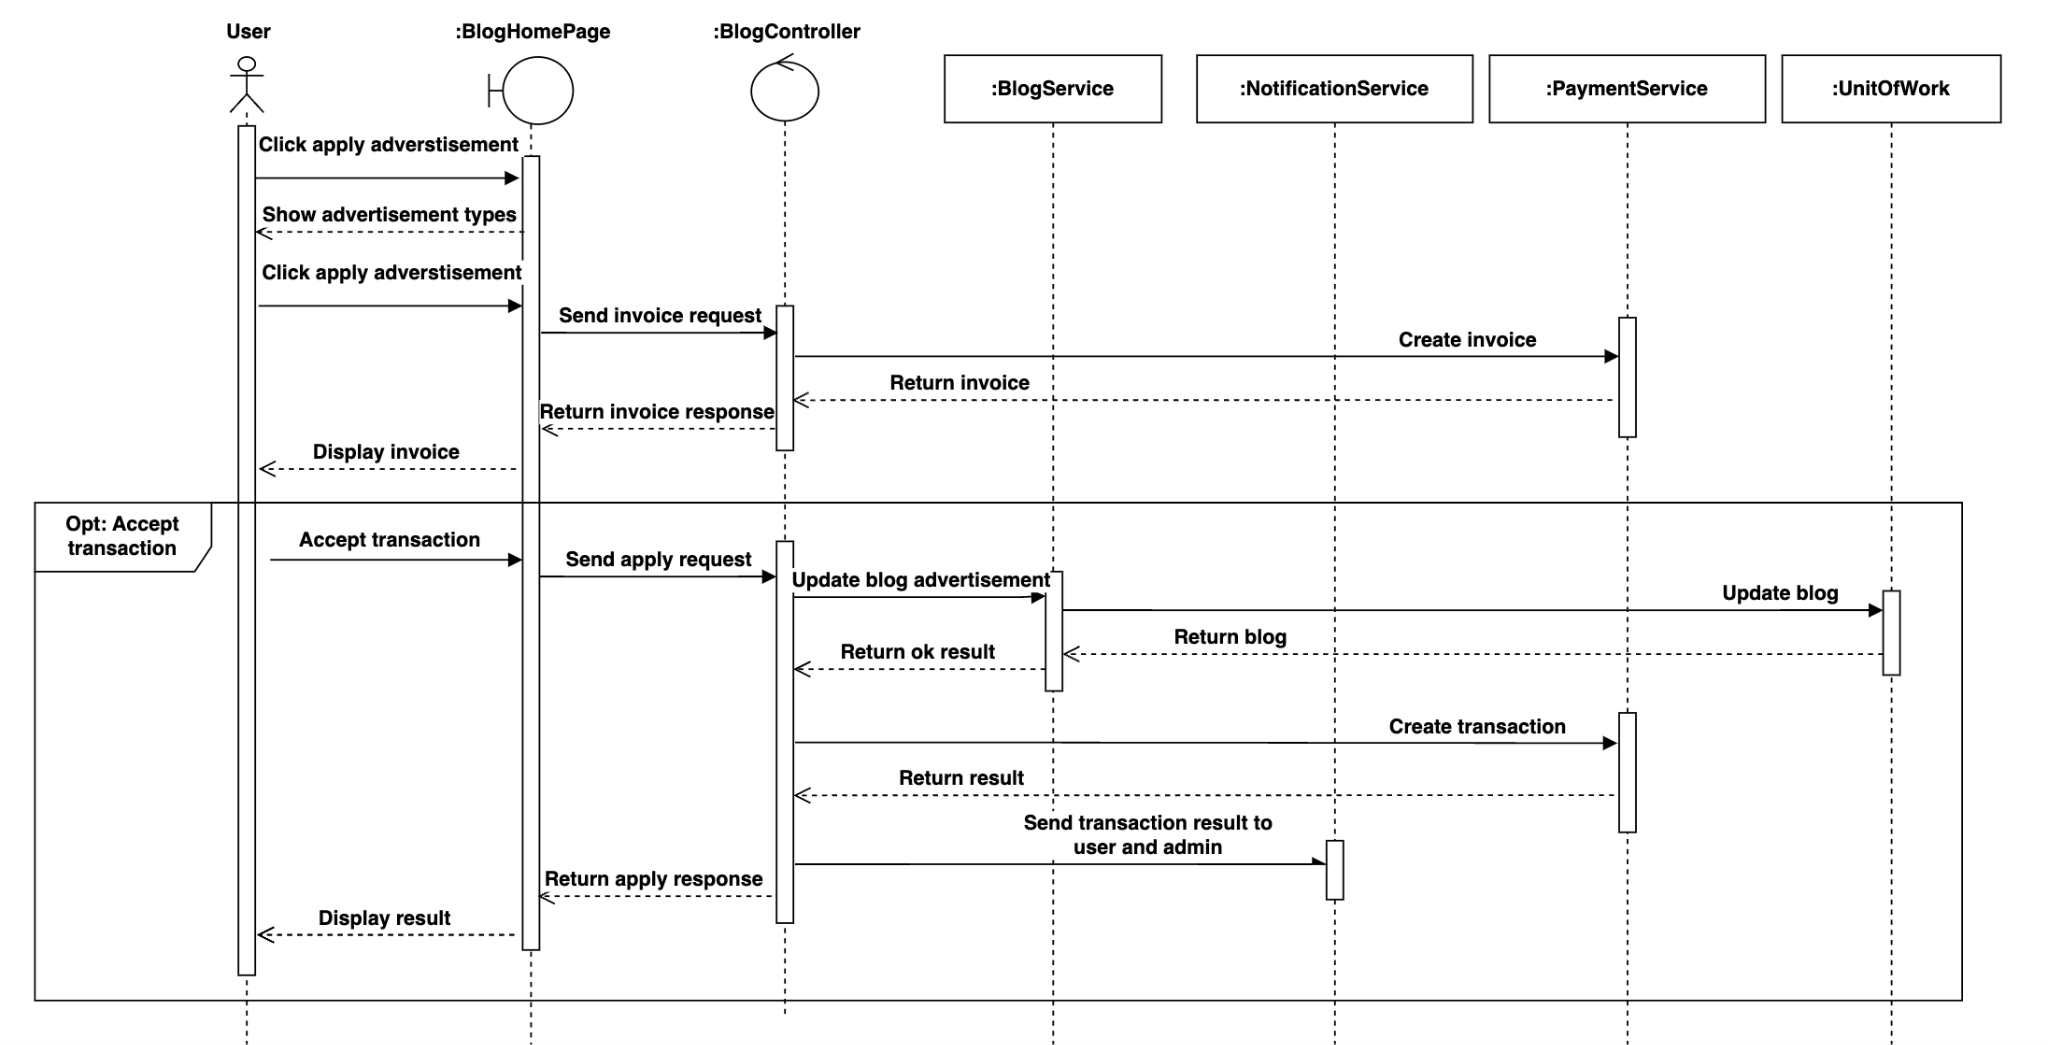
\includegraphics[width=0.9\textwidth]{Figures/payment_seq.png}
  \caption{Make payment sequence diagram}
  \label{fig:make-payment-seq}
\end{figure}


